\PassOptionsToPackage{table,xcdraw}{xcolor}

\documentclass[sigconf,review,anonymous]{acmart}
\acmConference[ESEC/FSE 2022]{The 30th ACM Joint European Software Engineering Conference and Symposium on the Foundations of Software Engineering}{14 - 18 November, 2022}{Singapore}

%\documentclass[sigconf,review,anonymous]{acmart}
%\acmConference[ESEC/FSE 2021]{The 29th ACM Joint European Software Engineering Conference and Symposium on the Foundations of Software Engineering}{23 - 27 August, 2021}{Athens, Greece}

%\acmConference[ICSE 2022]{The 44th International Conference on Software Engineering}{May 21–29, 2022}{Pittsburgh, PA, USA}

%\documentclass[sigconf,review, anonymous]{acmart}
%\documentclass[sigconf]{acmart}

\usepackage{booktabs}   %% For formal tables:
                        %% http://ctan.org/pkg/booktabs
\usepackage{subcaption} %% For complex figures with subfigures/subcaptions
                        %% http://ctan.org/pkg/subcaption
\usepackage{array}
\usepackage{amsmath,amsfonts}
\usepackage{algorithm}
\usepackage[noend]{algpseudocode}
%\usepackage{algorithmic}
\usepackage{graphicx}
\usepackage{textcomp}
\usepackage{float}
\usepackage{listings}
\usepackage{xspace}
\usepackage{multirow}
\usepackage{amsthm}
\newtheorem{definition}{Definition}
\usepackage{balance}

\usepackage[skins]{tcolorbox}

\usepackage{xcolor,pifont}
\newcommand*\colourcheck[1]{%
	\expandafter\newcommand\csname #1check\endcsname{\textcolor{#1}{\ding{52}}}%
}
\colourcheck{blue}
\colourcheck{green}
\colourcheck{red}

\newtcolorbox{myframe}[2][]{%
  enhanced,colback=white,colframe=black,coltitle=black,
  sharp corners,
  toprule=1.0pt,
  rightrule=0.3pt,
  leftrule=0pt,
  bottomrule=0pt,
  fonttitle=\itshape\scshape\large,
  left=0pt,right=5pt,top=5pt,bottom=3pt,
  attach boxed title to top right={yshift=-0.3\baselineskip-0.4pt,xshift=-5mm},
  boxed title style={tile,size=minimal,left=0.2mm,right=0.5mm,
    colback=white,before upper=\strut},
  title=#2,#1
}

%\newcommand{\code}[1]{{\footnotesize\textsf{#1}}}

\newcommand{\tool}{\textsc{UTango}\xspace}

\newcommand{\mvpdg}{$\delta$-PDG$^{i,j}$}

\newtheorem{Definition}{Definition}
\newtheorem{Claim}{Claim}
\newtheorem{Lemma}{Lemma}
\newtheorem{Theorem}{Theorem}

\newcolumntype{L}[1]{>{\raggedright\arraybackslash}p{#1}}
\newtheorem{observation}{Observation}
\newtheorem{property}{Property}
\newcommand{\code}[1]{{\footnotesize\texttt{#1}}}
\usepackage{amsthm}
 \definecolor{dkgreen}{rgb}{0,0.6,0}
\definecolor{gray}{rgb}{0.5,0.5,0.5}
\definecolor{mauve}{rgb}{0.58,0,0.82}
\lstset{frame=tb,
  language=Java,
  aboveskip=3mm,
  belowskip=3mm,
  showstringspaces=false,
  columns=flexible,
  basicstyle={\small\ttfamily},
  numbers=left,
  numberstyle=\tiny\color{gray},
  keywordstyle=\color{blue},
  commentstyle=\color{dkgreen},
  stringstyle=\color{mauve},
  breaklines=true,
  breakatwhitespace=true,
  tabsize=4
}



\begin{document}

%\title[{\tool}: Deep Fault Localization with Code Coverage Representation Learning]{{\tool}: Deep Fault Localization with Code Coverage Representation Learning}

\title[Untangling Commits with Context-aware, Graph-based, Code Change Clustering Learning Model]{{\tool}: Untangling Commits with Context-aware,\\ Graph-based, Code Change Clustering Learning Model}

%Context-aware
%ML
%Clone-aware
%Graph-based


%%%---- AUTHORS BLOCK ------

\setcopyright{none}

\settopmatter{printacmref=false, printfolios=false}

\renewcommand\footnotetextcopyrightpermission[1]{} % removes footnote with conference information in first column


%(1) present information sorted in a way that a CNN can "see" patterns
%discriminating between faulty and non faulty statements more easily;

%(2) identify the actual crash statement to the network;

%(3) present more information to the deep neural network in the form of
%a summary of data dependence for each statement as well as source
%embedding; and

%(4) the suspiciousness of a statement is seen taking into account
%relationships to other statement, as opposed to a statement by itself”



%\input{sections/abstract}
\begin{abstract}
During software evolution, developers make several changes and commit
them into the repositories. Unfortunately, many of them tangle
different purposes, both hampering program comprehension and reducing
separation of concerns. Automated approaches with deterministic
solutions have been proposed to untangle commits.
%Unlike the state-of-the-art, deterministic untangling approaches,

In this work, we present {\bf \tool}, a machine learning (ML)-based
approach that learns to untangle the changes in a commit.
%
We develop a {\em novel code change clustering learning model} that
learns to cluster the code changes, represented by the embeddings,
into different groups with different concerns.
%
We adapt the agglomerative clustering algorithm into a
supervised-learning clustering model operating on the learned code
change embeddings via trainable parameters and a loss function in
comparing the predicted clusters and the correct ones during training.
%
%Another key idea of {\tool} is
To facilitate our clustering learning model, we develop a {\em
context-aware, graph-based, code change representation learning
model}, leveraging Label, Graph-based Convolution Network to produce
the {\em contextualized embeddings for code changes}, that integrates
program dependencies and the surrounding contexts of the changes. The
contexts and cloned code are also explicitly represented, helping
{\tool} distinguish their concerns.
%
\textcolor{red}{Our empirical evaluation on a public C\# dataset
with 21k commits and 1,612 concerns shows that it achieves the
accuracy of 28.6\%--462.5\%, relatively higher than the
state-of-the-art approaches in clustering the changed code. We also
evaluated {\tool} in a Java dataset with {\bf XX} commits. The result shows
that it achieves {\bf XX.X\%} relatively higher accuracy than the
state-of-the-art approach.}

%Our sensitivity also shows that all designed components in {\tool}
%contributes positively to its high accuracy.}
\end{abstract}

%\textcolor{red}{Our empirical evaluation on a real-world C\# dataset
%with 21k commits and 1,612 concerns shows that it achieves the
%accuracy of XX.X\%--XX.X\% and YY.Y\%--YY.Y\% relatively higher than
%the state-of-the-art approaches in cross-project and within-project
%settings. We also evaluated {\tool} in a Java dataset with XX
%commits. The results show that it achieves accuracy XX.X\% relatively
%higher than the state-of-the-art approach.  Our sensitivity also shows
%that all designed components in {\tool} contributes positively to its
%high accuracy.}

%We develop a novel code change representation learning model
%leveraging Graph-based Convolution Network to build the vector
%representations for the changes, which integrate program dependencies,
%the surrounding contexts of the changes, as well as the code clone
%relationships.

%\settopmatter{printacmref=true, printccs=true, printfolios=false}

%\begin{CCSXML}
%<ccs2012>
%<concept>
%<concept_id>10011007.10011006.10011073</concept_id>
%<concept_desc>Software and its engineering~Software maintenance tools</concept_desc>
%<concept_significance>500</concept_significance>
%</concept>
%</ccs2012>
%\end{CCSXML}

%\ccsdesc[500]{Software and its engineering~Software maintenance tools}

%\keywords{Deep Learning; Automated Program Repair; Context-based Code Transformation Learning}


\maketitle

\section{Introduction}
\label{intro:sec}

During software evolution, developers make several changes over time
and commit them into a source code repository. The changes to the
source files that are committed to the repository at the same
transaction are often referred to as a {\em change set} or a {\em
  commit}. In an ideal world, each commit should be about one purpose
or concern regarding the programming task at hand.  Unfortunately, Tao
{\em et al.}~\cite{tao-fse12}, Kim {\em et
  al.}~\cite{kim-emse16,kim-msr13}, and Hill {\em et
  al.}~\cite{hill-tse12} have reported that many change sets or
commits tangle different concerns including the changes for
bug-fixing, refactoring, enhancements/improvements, or
documentation. Such change sets are called {\em tangled code changes}
or {\em tangled commits}~\cite{kim-emse16,kim-msr13}. The prior work
reported two reasons for tangled commits: time pressure in committing
the changes, and unclear boundaries between the concerns for code
changes~\cite{flexeme-fse20}.

Tangled commits pose several issues in software development. First,
they affect software quality in both hampering program
comprehension~\cite{tao-fse12} and reducing separation of concerns in
code changes~\cite{flexeme-fse20}. Second, the tangled commits
might contain the bug-fixing changes for one bug that are mixed with
the fixes for other bugs as well as different types of changes for
refactoring, enhancements, or
documentation~\cite{kim-emse16,kim-msr13,nguyen-issre13}. Those
tangled commits have negative impacts on the accuracy of bug
prediction or bug localization models that rely on the data mined from
the version histories~\cite{kim-emse16,kim-msr13}. Those models 
consider an entire commit as for fixing or non-fixing, thus,
are significantly affected by the tangled commits.

Recognizing the need of the tools that untangle, i.e., decompose a
commit into untangle changes, several researchers have proposed
different approaches that can be broadly classified into two
categories: {\em mining software repositories}, and {\em program
  analysis}.

First, earlier approaches leverage the {\em mining software
  repositories (MSR)} techniques. Herzig {\em et
  al.}~\cite{kim-msr13,kim-emse16} utilize a confidence voter
technique together with agglomerative clustering on the change
operations to untangle the commits.
%Each confidence voter is responsible for an important aspect
%including call-graphs, change couplings, data dependencies, and
%distance measures.
However, the voters are independent, thus, do not reflect well the
interdependency nature of program elements under change. In contrast,
Kirinuki {\em et al.}~\cite{higo-apsec16, higo-icpc14} rely on the
histories of the co-changes to split the tangled code changes before
they are committed. However, they do not consider the dependencies
among the changes such as data or control dependencies. Dias {\em et
  al.}~\cite{dias-saner15} also use confidence voters, but on the
fine-grained change events in an IDE. The scores are converted into
the similarity ones via a Random Forest Regressor, which are used in
the agglomerative clustering to partition the tangled changes.  The
second category of untangling approaches leverage the {\em static
  analysis} techniques. Roover {\em et al.}~\cite{roover-scam18} use
program slicing to segment a commit across a Program Dependency Graph
(PDG).  However, they are limited handling interprocedural and
cross-file dependencies. Barnett {\em et al.}~\cite{barnett-icse15}
utilize def-use chains, and cluster them. If the def-use chain all
fall into a method, it is considered as trivial, otherwise,
non-trivial. Because igoring the trivial clusters, it can miss tangled
concerns. To improve over that, Flexeme~\cite{flexeme-fse20} uses
multi-version PDG augmented with name/lexeme flows in the edges, and
applies Agglomerative Clustering using Graph Similarity on the graph
to untangle its commits.


\section{Motivation}
\label{motiv:sec}

\subsection{Motivating Examples}
\label{exe:sec}

\begin{figure}[t]
	\centering
	\lstset{
		numbers=left,
		numberstyle= \tiny,
		keywordstyle= \color{blue!70},
		commentstyle= \color{red!50!green!50!blue!50},
		frame=shadowbox,
		rulesepcolor= \color{red!20!green!20!blue!20},
                rulecolor= \color{black},
		xleftmargin=1.5em,xrightmargin=0em, aboveskip=1em,
		framexleftmargin=1.5em,
                numbersep= 5pt,
		language=Java,
    basicstyle=\scriptsize\ttfamily,
    numberstyle=\scriptsize\ttfamily,
    emphstyle=\bfseries,
                moredelim=**[is][\color{red}]{@}{@},
		escapeinside= {(*@}{@*)}
	}
	\begin{lstlisting}[]
Commit r1192 ``Fixes NPE and implements indentation of XML elements.''
 /trunk/jhotdraw8/src/main/java/org/jhotdraw8/draw/Drawing.java
 ...
(*@{\color{red}{- public final static Key<List<URI>> AUTHOR\_STYLESHEETS = new SimpleFigureKey<> ("authorStylesheets", List.class, new Class<?>[]\{URI.class\}},...,}@*)(*@{\color{violet}{ null);}@*)
(*@{\color{cyan}{+ public final static Key<List<URI>> AUTHOR\_STYLESHEETS = new SimpleFigureKey<> ("authorStylesheets", List.class, new Class<?>[]\{URI.class\}},...,}@*)(*@{\color{violet}{ Collections.emptyList());}@*)
 ...
(*@{\color{red}{- public final static Key<List<URI>> USER\_AGENT\_STYLESHEETS = new SimpleFigureKey<>("userAgentStylesheets", List.class, new Class<?>[]{URI.class},...,}@*)(*@{\color{violet}{ null);}@*)
(*@{\color{cyan}{+ public final static Key<List<URI>> USER\_AGENT\_STYLESHEETS = new SimpleFigureKey<> ("userAgentStylesheets", List.class, new Class<?>[]\{URI.class\},...,}@*)(*@{\color{violet}{ Collections.emptyList());}@*)
 ...
(*@{\color{red}{- public final static Key<List<String>> INLINE\_STYLESHEETS=new SimpleFigureKey <>("inlineStylesheets",List.class,new Class<?>[]\{String.class\},.,}@*)(*@{\color{violet}{null);}@*)
(*@{\color{cyan}{+ public final static Key<List<String>> INLINE\_STYLESHEETS=new SimpleFigureKey <>("inlineStylesheets", List.class, new Class<?>[]\{String.class\},...,}@*)(*@{\color{violet}{ Collections.emptyList());}@*)
//--------------------------------------------------------------------------
 /trunk/jhotdraw8/src/main/java/org/jhotdraw8/draw/io/SimpleXmlIO.java
 public Document toDocument(Drawing internal,Collection<Figure> selection)..{
   for (Figure child : ordered) {
   (*@{\color{red}{-            writeNodeRecursively(doc, docElement, child);}@*)
   (*@{\color{red}{-\}}@*)
   (*@{\color{red}{-          docElement.appendChild(doc.createTextNode("..."));}@*)
   (*@{\color{cyan}{+            writeNodeRecursively(doc, docElement, child, linebreak);}@*)
   (*@{\color{cyan}{+\}}@*)
   (*@{\color{cyan}{+          docElement.appendChild(doc.createTextNode(linebreak));}@*)
   return doc; ...
}
	\end{lstlisting}
        \vspace{-15pt}
        \caption{A Tangled Commit at r1192 of JHotDraw}
        \vspace{-6pt}
        \label{fig:motiv-cc}
\end{figure}

\begin{figure}[t]
	\centering
	\lstset{
		numbers=left,
		numberstyle= \tiny,
		keywordstyle= \color{blue!70},
		commentstyle= \color{red!50!green!50!blue!50},
		frame=shadowbox,
		rulesepcolor= \color{red!20!green!20!blue!20} ,
		xleftmargin=1.5em,xrightmargin=0em, aboveskip=1em,
		framexleftmargin=1.5em,
                numbersep= 5pt,
		language=Java,
    basicstyle=\scriptsize\ttfamily,
    numberstyle=\scriptsize\ttfamily,
    emphstyle=\bfseries,
                moredelim=**[is][\color{red}]{@}{@},
		escapeinside= {(*@}{@*)}
	}
	\begin{lstlisting}[]
  Commit r1023 ``Fixes bugs in FigureStyleManager''
  /trunk/jhotdraw8/src/main/java/org/jhotdraw8/draw/Drawing.java
   
(*@{\color{red}{-    public final static Key<List<URI>> AUTHOR\_STYLESHEETS = new SimpleFigureKey<> ("authorStylesheets", List.class, }@*)(*@{\color{violet}{"<URI>",}@*)(*@{\color{red}{,..., null);}@*)
(*@{\color{cyan}{+     public final static Key<List<URI>> AUTHOR\_STYLESHEETS = new SimpleFigureKey<> ("authorStylesheets", List.class, }@*)(*@{\color{violet}{new Class<?>[]\{URI.class\},}@*)(*@{\color{cyan}{..., null);}@*)

(*@{\color{red}{-    public final static Key<List<URI>> USER\_AGENT\_STYLESHEETS=new SimpleFigureKey <>("userAgentStylesheets", List.class, }@*)(*@{\color{violet}{"<URI>",}@*)(*@{\color{red}{..., null);}@*)
(*@{\color{cyan}{+ public final static Key<List<URI>> USER\_AGENT\_STYLESHEETS=new SimpleFigureKey<> ("userAgentStylesheets", List.class, }@*)(*@{\color{violet}{new Class<?>[]\{URI.class\},}@*)(*@{\color{cyan}{..., null);}@*)

(*@{\color{red}{-    public final static Key<List<String>> INLINE\_STYLESHEETS=new SimpleFigureKey <>("inlineStylesheets", List.class, }@*)(*@{\color{violet}{"<String>",}@*)(*@{\color{red}{..., null);}@*)
(*@{\color{cyan}{+    public final static Key<List<String>> INLINE\_STYLESHEETS=new SimpleFigureKey <>("inlineStylesheets",List.class,}@*)(*@{\color{violet}{new Class<?>[]\{String.class\},}@*)(*@{\color{cyan}{.,null);}@*)
	\end{lstlisting}
        \vspace{-15pt}
        \caption{Same Statements as in r1192 were Changed at r1023 of JHotDraw and Belonged to Only One Concern}
        \vspace{-6pt}
        \label{fig:history}
\end{figure}

%\caption{Changes of Same Concern in r1023 of JHotDraw}

%public static ParserResult<T> Build<T>(...) {
%  ...
%  select
%(*@{\color{red}{  - sp.Value.MapValueOrDefault(}@*)
%(*@{\color{red}{  - \quad   v => v,}@*)
%(*@{\color{red}{  - \quad  sp.Specification.DefaultValue.MapValueOrDefault(}@*)
%(*@{\color{red}{  - \quad \quad   d => d,}@*)
%(*@{\color{cyan}{  + sp.Value.GetValueOrDefault(}@*)
%(*@{\color{cyan}{  + \quad sp.Specification.DefaultValue.GetValueOrDefault(}@*)
%(*@{\color{cyan}{   \quad  sp.Specification.ConversionType.CreateDefaultForImmutable()))).ToArray();}@*)
%  var immutable = (T)ctor.Invoke(values);
%  return immutable;
%}

Let us present the real-world examples to motivate {\tool}.
%our motivation.
Figure~\ref{fig:motiv-cc} shows the changes at the commit
r1192 of the JHotDraw project with the log {\em ``Fixes NPE and
  implements indentation of~XML elements''}. This is a tangled commit
with two concerns/purposes: 1) the fix for Null Pointer Exception
occurred at lines 4,7, and 10 of the \code{Drawing} class (the
\code{null} argument was replaced with
\code{Collections.empty\-List()}); 2) the implementation of the indentation
of XML elements occurred at lines 16--18, and a few other lines of the
\code{SimpleXmlIO} class and one line in the \code{Drawing} class (not
shown).

Figure~\ref{fig:history} shows the changes committed at r1023 earlier
in JHotDraw. The changes occurred at the same lines 4, 7, and 10 of
the \code{Drawing} class as the commit at r1192 in
Figure~\ref{fig:motiv-cc}. However, the commit at r1023 was for only
one concern as stated in the commit log {\em ``Fixes bugs in
  FigureStyleManager''}. This example motivates us to build a ML model
to learn from the co-changes for the same concern in the version
history to untangle the current commit.

%Figure~\ref{fig:motiv-cc} shows an example from the experimental
%dataset in a prior work~\cite{flexeme-fse20}. This commit has three
%changed statements at lines 4, 10, and 17 of the methods
%\code{MapValuesImpl}, \code{WithNextValue}, and \code{Build}.  The
%method \code{MapValueOrDefault} was renamed to
%\code{GetValueOr\-Default}, causing the changes to the call sites.
%These changes are deemed by the developers as serving the same
%concern/purpose of enhancing type resolution in the parser. {\em These
%  statements have been changed for the same concern} of fixing the
%value parsing in a past commit. This motivates us to build a ML model
%to learn from the co-changes for the same concern in the version
%history to untangle the commits.
%---------------------

%Tien
%For this example, the untangling approaches relying on the PDGs or
%program slices within individual methods cannot cluster the changed
%statements into a group.

%(e.g.,~\cite{flexeme-fse20},~\cite{roover-scam18})

\vspace{3pt}
\noindent {\bf Observation 1 [Learn to Cluster Code Changes].} {\em
  History of the co-changed statements with the same concern could be
  a good source for a machine learning model to learn to cluster the
  changed statements, thus, untangling the current commits}.

\begin{figure}[t]
	\centering
	\lstset{
		numbers=left,
		numberstyle= \tiny,
		keywordstyle= \color{blue!70},
		commentstyle= \color{red!50!green!50!blue!50},
		frame=shadowbox,
		rulesepcolor= \color{red!20!green!20!blue!20} ,
		xleftmargin=1.5em,xrightmargin=0em, aboveskip=1em,
		framexleftmargin=1.5em,
                numbersep= 5pt,
		language=Java,
    basicstyle=\scriptsize\ttfamily,
    numberstyle=\scriptsize\ttfamily,
    emphstyle=\bfseries,
                moredelim=**[is][\color{red}]{@}{@},
		escapeinside= {(*@}{@*)}
	}
	\begin{lstlisting}[]
public void mousePressed(MouseEvent evt) { 
  ...//SelectionTool.java
(*@{\color{red}{- if (figure != null) {}@*)
(*@{\color{cyan}{+ if (figure != null}@*) && (*@{\color{cyan}{figure.isSelectable()) {}@*)
       newTracker = createDragTracker(figure);
    } else {
       if (! evt.isShiftDown()) {...}
}
//--------------------------------------------------------------------------
protected void updateHoverHandles(DrawingView view, Figure f) {
  ...// SelectAreaTracker.java
  figure = f;
(*@{\color{red}{- if (figure != null) {}@*)
(*@{\color{cyan}{+ if (figure != null}@*) && (*@{\color{cyan}{figure.isSelectable()) {}@*)
      hoverHandles.addAll(figure.createHandles(-1)); ...
}
	\end{lstlisting}
        \vspace{-15pt}
        \caption{Same Change in 2 Contexts for Diff. Concerns (r463)}
        \vspace{-6pt}
        \label{fig:motiv-context}
\end{figure}

% \caption{Same Change in Two Contexts for Different Concerns in the Commit r463 of JHotDraw}

Figure~\ref{fig:motiv-context} shows another example in JHotDraw
project. At the commit r463, two changes at line 3 and line 13 are
exactly the same with the addition of \code{figure.isSelectable()} to
check whether a figure is selectable or not. However, those {\em two
  exact changes} occurred in two different methods \code{mousePressed}
and \code{updateHoverHandles} for two different concerns/purposes as
noted in the commit log. Line 4 was aimed to fix the tracking of a
dragging object as the mouse is pressed ({\em ``Fixed bug where
  setSelectable() on a dragging figure did not work''}).  Line 14 was
a fix for a different bug as the hovered object needs to be selected
({\em ``Selection classes now check the flag on the hovering figures
  to be selected.''}). The addition of \code{figure.isSelectable()} is
common for checking if a figure is selectable in the two tasks of
dragging and hovering a figure. Without the surrounding contexts,
one could not tell that they are for different purposes.

\vspace{3pt}
\noindent {\bf Observation 2 [Context].} {\em The surrounding context
  consisting of un-changed code is crucial to determine the
  concern of a change. The same change in two 
  contexts could be for different concerns}.

Figure~\ref{fig:motiv-cc} also gives us another interesting
observation. The changes at lines 4, 7, and 10 are exactly the same to
fix the NPE: \code{null} $\rightarrow$ \code{Collections.emptyList()}.
The three statements are cloned code of one another to support for
different stylesheets (author, user agent, and inline stylesheets).
In fact, the changes in Figure~\ref{fig:history} also occurred at the
cloned statements. The three changes belong to the same
concern/purpose since they serve as a fix for the same logic despite
that there is no program dependency among them. The existing
untangling
approaches~\cite{flexeme-fse20,smartcommit-fse21,roover-scam18,barnett-icse15}
that require the explicit program dependencies among the changes with
the same purpose will not classify these committed code as belonging
to the same concern.

%Figure~\ref{fig:motiv-clone} shows another example on the two
%fragments of cloned code for two different security types (Crypto and
%Equity) and markets (GDAX and USA). They were fixed in the same manner
%at line 4 and line 13. The two changes were in the same fix to convert
%the usage of \code{PortfolioSelection} into that of
%\code{UniverseSelection}, and the usage of
%\code{ManualPortfolioSelectionModel} into that of
%\code{ManualUniverseSelection\-Model} in the process of {\em ``setting
%  algorithm framework models''}.

\vspace{2pt}
\noindent {\bf Observation 3 [Implicit Dependencies].} {\em Two
  fragments of cloned code have the same/similar logic, thus, have
  implicit dependencies, and could be modified in the same manner to
  serve the same concern.}

%\vspace{-12pt}
\subsection{Key Ideas}
\label{ideas:sec}

From the motivation, we propose {\tool} with the following
ideas.

%{\bf Key Idea 1 [Code Change Representation Learning with Graph
%    Convolution Network (GCN)]}.

{\bf Key Idea 1 [Code Change Clustering Learning Model]}. Instead of
deciding a deterministic clustering criterion on the concrete
artifacts (PDGs, program slices, code changes, operations, or change
graphs), from Observation 1, we build an ML model to untangle the
commits by learning to cluster code~changes represented by embeddings,
w.r.t. different concerns. The model learns from the~history of the
co-changed statements in the same commits for the same concerns, and
applies to cluster the changes in the current commit.  We also modify
an agglomerative clustering algorithm into a~super\-vised-learning
clustering model via trainable parameters and a loss function to
compare the predicted clusters and the correct ones.

{\bf Key Idea 2 [Context-aware, Graph-based Representation Learning
    for Code Changes].} We design a context-aware, graph-based,
representation learning model to {\em learn the contextualized
  embeddings (vectors) for the code changes} that integrates {\em
  program dependencies} among the program elements, and the {\em
  contexts} of~code changes. We train a Label, Graph-based Convolution
Network~\cite{label-gcn} to learn the embeddings and learn the
clusters from the history of changed code for the same concerns.
For prediction, we apply supervised-learning agglomerative
clustering on the embeddings of code changes to produce the clusters
to untangle the commit. We expect that supervised-learning clustering
on vectors is more effective than on the above artifacts since the
embeddings capture~richer information integrated from the
dependencies and contexts.


{\bf Key Idea 3 [Explicit Context Representation as a Weight to
    Compute Vectors for Code Changes]}. As in Observation 2, the
contexts of the code changes can help distinguish their concerns in
the commits. We represent code changes and the surrounding context of
a change via the multi-version program dependence~graph,
$\delta$-PDG~\cite{flexeme-fse20}, consisting of the elements of both
versions before and after the changes, and program dependencies. The
context is defined as the surrounding nodes of the changed statement
node in that graph. The Label-GCN is used to model the statements and their
dependencies in $\delta$-PDG and to learn the vector
representation of the context for a change. The context vectors are
then used as weights in learning contextualized embeddings for the
code changes.

{\bf Key Idea 4 [Implicit Dependencies among Cloned Code]}. As in
Observation 3, the cloned code exhibits implicit dependencies with
regard to whether they can be changed in the same commits for the same
concerns. Thus, during the process of producing the final
result, we also integrate the code clone relationships to
adjust the clusters produced by the clustering learning model.

%Thus, the GCN model can learn the embeddings of the code changes with
%the consideration of the cloned code.





\section{Approach Overview}
\label{overview:sec}

\subsection{Important Concepts}
\label{concepts:sec}



Let us first define some important concepts used in {\tool}.

%First, we formally define the PDG, multi-version PDG, changed/unchanged statements, and context to conduct our approach's overview. Within these definitions, We re-use the definition of program dependency graph and multi-version program dependency graph from Partachi et al.'s research \cite{flexeme-fse20}.

\begin{Definition}[Program Dependence Graph]
The \textbf{program dependency graph (PDG)}~\cite{pdg} is a directed
graph with a set $N$ of nodes and a set $E$ of edges such that each
node $n \in N$ represents a program statement or a conditional
expression; each edge $e \in E$ represents the data or control flow
among the statements.
\end{Definition}

%s.t. each node 𝑛 ∈ 𝑁 is annotated with either a program statement or a
%conditional expression; each edge 𝑒 ∈ 𝐸 has an optional annotation
%representing the name or the data that flows along it, and a kind that
%describes the relationship type: data or control.

Figure~\ref{fig:multi-version-pdg} shows the code change in a commit
in which the statement \code{int next = i + 1;} is replaced by
\code{var next = i + 1;}. Figure~\ref{fig:multi-version-pdg} (a) and
(b) display the PDGs of the method \code{FormatYear} before and after
the change. All the nodes of the PDG before the change are marked with
$i$, and those of the PDG after the change are marked with $j$.

%As shown in figure \ref{fig:multi-version-pdg}, the graph with all nodes labeled $i$, and the graph with all nodes labeled with $j$ is the PDG for the version $i$ and version $j$ of the method $FormatYear$. After having these two PDGs, we can define the multi-version program dependency graph. $\delta$-PDG$^{i,j}$

\begin{figure}[t]
	\centering
	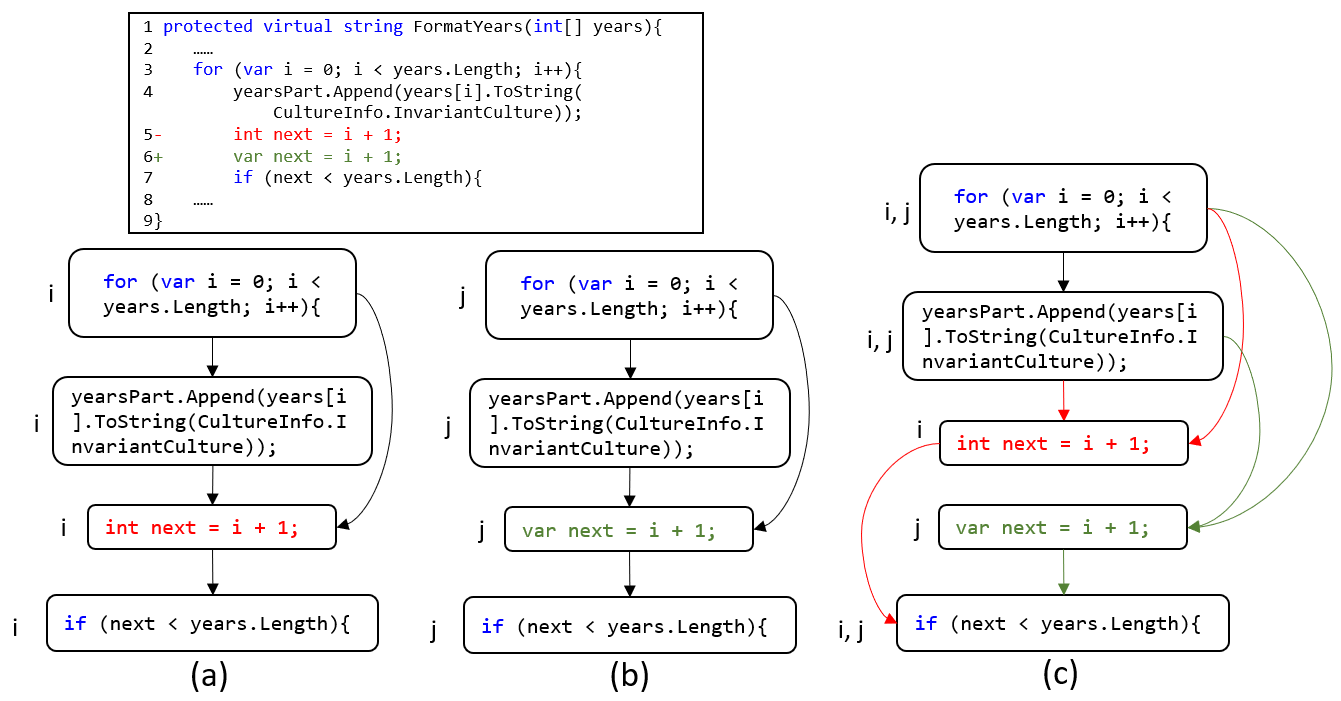
\includegraphics[width=3.5in]{figures/multi-version-graph-3.png} %5.3
	\vspace{-18pt}
	\caption{Multi-Version Program Dependence Graph}
	\label{fig:multi-version-pdg}
\end{figure}

\begin{figure*}[t]
	\centering
 	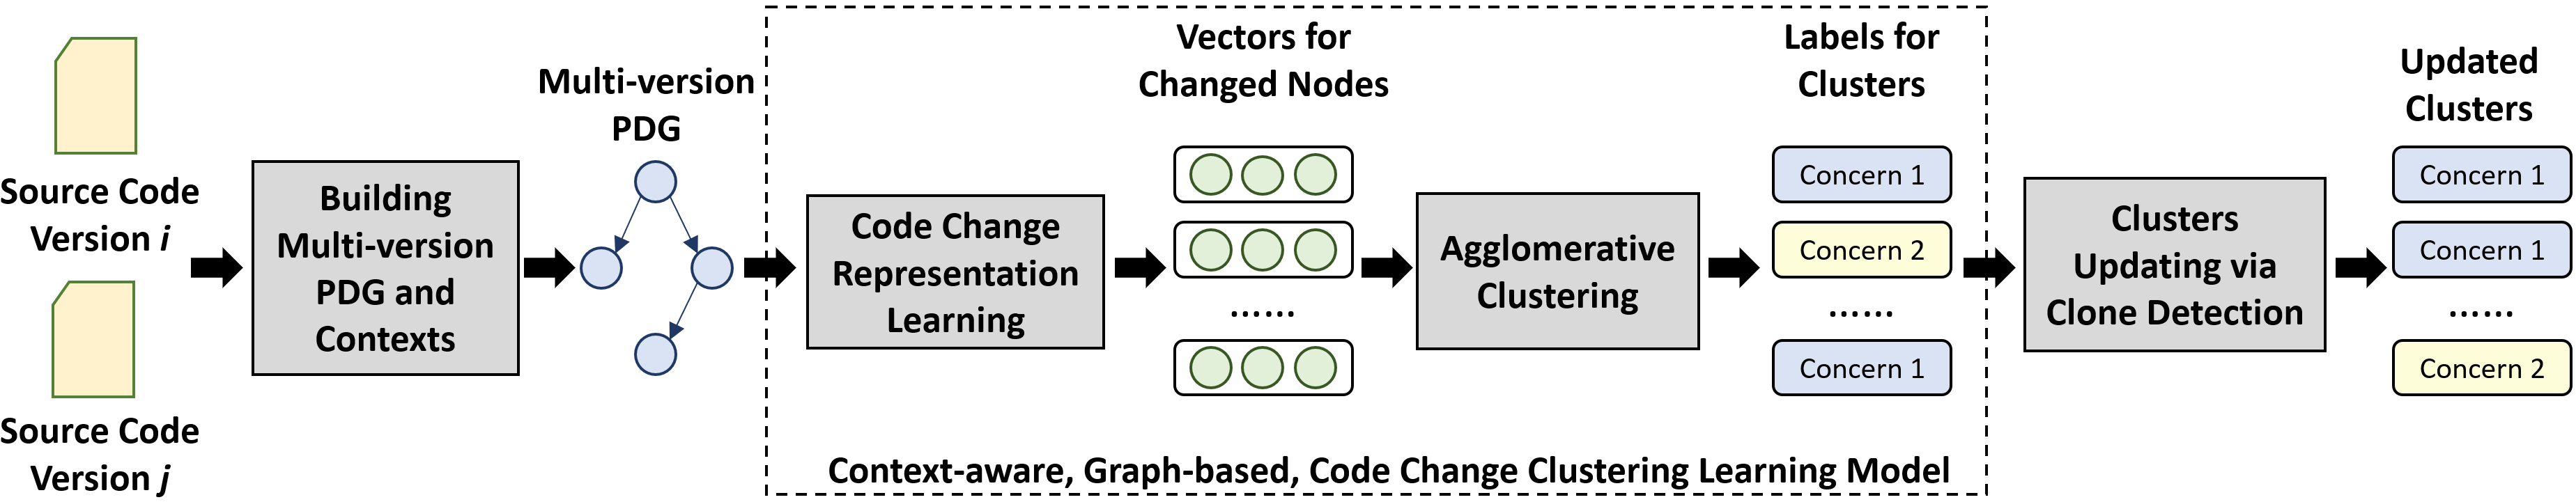
\includegraphics[width=6.8in]{figures/overview-3.png}
	\vspace{-6pt}
	\caption{{\tool}: Architecture Overview}
	\label{fig:overview}
\end{figure*}


\begin{Definition}[Multi-version Program Dependence Graph] ({\bf $\delta$-PDG}).
A {\mvpdg} is a directed graph generated from the disjoint union of
all nodes and edges in the PDGs at versions $i$
and~$j$~\cite{flexeme-fse20}.
%
%  The \textbf{multi-version program dependency graph (Multi-version PDG$^{i,j}$)} is a directed graph that generated from the disjoint union of all nodes and edges between the version $i$ and version $j$. $\delta-PDG^{i,i}$ is the PDG at the version $i$.
\end{Definition}

Figure~\ref{fig:multi-version-pdg}(c) displays the multi-version
PDG$^{i,j}$ ({\mvpdg}) that are built from the two
versions $i$ and $j$ of the method \code{FormatYear} before and after
the change. In {\mvpdg}, the nodes labeled with either $i$
or $j$ appear only in the PDG for the version $i$ or the version $j$.
The nodes labeled with $i$,$j$ appear in the PDGs at both the
versions.

%figure \ref{fig:multi-version-pdg}, the third graph that contains the nodes labeled with $i$, $j$, and $i, j$ is the multi-version PDG$^{i,j}$ combined from the two PDGs for version $i$ and $j$ for the method $FormatYear$. In this graph, the nodes labeled with $i$ or $j$ are the nodes that appeared only in the PDG for version $i$ or $j$. And the nodes labeled with $i, j$ are the nodes that appeared in the PDG for both version $i$ and $j$. With the multi-version PDG$^{i,j}$, we make the definition for the changed/unchanged statements.

\begin{Definition}[Changed/Un-changed Nodes]
In the multi-version PDG, $\delta$-PDG$^{i,j}$ for the versions before
and after the change, the changed nodes represent the changed
statements, and are labeled with either $i$ or $j$, while the
un-changed nodes are labeled with $i,j$.
%The \textbf{changed statements} between version $i$ and $j$ are the statements that are added or deleted to changed the code from version $i$ to version $j$. The modification on an existing statement in version $i$ is regarded as a new statement addition with an old statement deletion. The \textbf{un-changed statements} between version $i$ and $j$ are the statements that keep the same in both version $i$ and version $j$.
\end{Definition}

In Figure~\ref{fig:multi-version-pdg}(c), the node labeled with $i$
represents the deleted statement, the node labeled with $j$ represents
the added one, while the nodes labeled with $i,j$ are for the un-changed
statements.

%The figure \ref{fig:multi-version-pdg} can be used an example to show both the changed and un-changed statements between version $i$ and $j$ for the method $FormatYear$. As seen in the multi-version PDG$^[i,j]$ for the method $FormatYear$, the statements $int\, next = i + 1;$ and $var\, next = i + 1;$ that are labeled with $i$ or $j$ are the changed statements between version $i$ and $j$ while the rest statements that are labeled with $i, j$ in the graph are the un-changed statements between version $i$ and $j$.

\begin{Definition}[Context]
The context $C$ of a changed node $n$ is a sub-graph of the
multi-version {\mvpdg} that includes all the un-changed nodes within
the $k$-hop neighbors of the changed node $n$, together with all the
inducing edges among them.
\end{Definition}

In Figure~\ref{fig:multi-version-pdg}(c), when $k$=1, the context for
the changed node/statement at line 5 consists of all three nodes
labeled with $i,j$ because they are one hop from the changed node for
`\code{int next = i + 1;}'.
%and \code{var next = i + 1;}.

%To better understand the context of a changed statement, we still use the figure \ref{fig:multi-version-pdg} as an example to explain. For the statement $int\, next = 1 + 1;$ in the multi-version PDG$^{i,j}$, we select the sub-graph that contains all $k$-hops neighbors as the context. When $k=1$, the sub-graph is built with three statements that labeled with $i, j$ in the multi-version PDG$^{i,j}$.




\subsection{Architecture Overview}
\label{arch-overview:sec}

%After having the definition for the important concepts, we use them to describe the overview of our approach. Within our approach, there are three main steps. We will introduce them one by one.

Figure~\ref{fig:overview} illustrates the overview of our model, {\tool}.

\subsubsection{{\bf Step 1. Building Multi-version PDG ($\delta$-PDG$^{i,j}$) and Contexts}}
The first step is to build the $\delta$-PDG$^{i,j}$ graph and extract
the context sub-graphs for each changed statement from the two
versions $i$ and $j$ before and after the changes. We adopt the
multi-version graph building algorithm from
Flexeme~\cite{flexeme-fse20}. Specifically, we first generate the PDGs
for both versions $i$ and $j$. We use the Git diff tool on the source
code to determine the changed and unchanged nodes for the
statements. The added nodes are kept in $\delta$-PDG$^{i,j}$ with the
labels $j$ as they appear in the newer version $j$. We also retain the
deleted nodes and use the label $i$ for them. The unchanged nodes
between the versions are matched by using string similarity among the
respective statements to filter the candidates and line-span proximity
to rank them. When considering the edge changes, we back-propagate the
delete nodes to the edges flowing into them. We also add all the unmatched
edges in the newer version $j$ to the multi-version PDG$^{i,j}$ as the
edges relevant to the added nodes. Details on building
$\delta$-PDG$^{i,j}$ can be found in~\cite{flexeme-fse20}.

After constructing $\delta$-PDG$^{i,j}$, for each changed node in the
graph, we collect all unchanged nodes within the $k$-hops and
all~their inducing edges to build a sub-graph as the context for the
changed~node. 
$\delta$-PDG$^{i,j}$ and the contexts for the changed nodes
will be used as the input for the next step.
%$\delta$-PDG$^{i,j}$ and the contexts are used in step 2.
This step of building $\delta$-PDG$^{i,j}$ and contexts is used in
both training and predicting processes.

%First, \tool accepts two versions $i$ and $j$ of source code. Following the existing study from Partachi et al. \cite{flexeme-fse20}, \tool firstly generates the PDGs for both the version $i$ and version $j$ for the source code. Next, to construct the multi-version PDG$^{i,j}$, \tool starts from the initial version $i$. \tool uses the PDGs and the Git diff tool on the source files to determine changed and unchanged nodes. Added nodes are introduced to the multi-version PDG$^{i,j}$ as they appear in the newer version $j$. \tool retains nodes deleted across the versions and uses a different label (label $i$) on the nodes to represent the deletion. The unchanged nodes between versions are matched by using string similarity to filter candidates and line-span proximity to rank them. When considering the edge changes, \tool back-propagates the delete nodes to edges flowing into them. Also, \tool considers and adds all unmatched edges in the newer version $j$ to the multi-version PDG$^{i,j}$ as the edges relevant to the added nodes. After having the constructed multi-version PDG$^{i,j}$, for each changed node in the graph, \tool collects all unchanged nodes within the $k$-hops and the edges between them to build a sub-graph as the context for the changed node. The multi-version PDG$^{i,j}$ and the context for each changed node in it will be used as the input for the next step.

\subsubsection{{\bf Step 2. Context-aware, Graph-based, Code Change Clustering Learning Model}} The task of this model is to {\em learn to cluster the code changes}, represented by
the changed nodes and corresponding contexts in {\mvpdg}. For
that, {\tool} first learns to construct the {\bf contextualized
  embeddings} to represent the code changes via our novel
{\bf context-aware, graph-based code change representation learning
  model}. In that model, to build the contextualized embeddings, we
leverage
%Label, Graph-based Convolution Network (GCN)
the Label-GCN~\cite{label-gcn} that can deal with the nodes with
multiple labels (used to denote the versions $i$, $j$) to learn the
representation vector $v$ for each node $n$ in the graph. For a
changed node $n_c$, we collect the vectors for the un-changed nodes in
the context for $n_c$ into a matrix. We use a fully connected layer to
convert the matrix into a vector $v_{ctx}$ to encode the contextual
information for the node $n_c$. The context vector $v_{ctx}$ is then
used as {\em a weight to represent the impact of the context on the
  learning to produce the final vector for the changed node $n_c$}.

%Tien
%The final vector $v'_c$ for $n_c$ is computed as the cross-product
%between the vector $v_c$ of $n_c$ computed from Label-GCN and the
%context vector $v_{ctx}$.



%By having the multi-version PDG$^{i,j}$ as the input, \tool firstly uses an advanced GCN model \cite{} that can deal with the nodes with different labels to learn the representation vectors $v_p$ for each node $n_p$ in the graph. For each changed node $n_c$ in $n_p$, \tool collects all unchanged node representation vectors in the context as a matrix. It then uses a fully connected layer to convert it to a vector $v_pc$ to represent all context information for the changed node $n_p$. Next, \tool generates the final representation vector $v'_p$ for changed node $n_p$ by using the cross product between $v_p$ and $v_pc$.

%With the representation vector $v'_p$ for all changed nodes $n_p$, \tool uses the agglomerative clustering algorithm to cluster the changed nodes into different concerns. Because the number of concerns in the real world commits is not known for \tool, \tool uses a trainable threshold for the linkage when merging the clusters. The output of this step is the clustering results $C$ from the clusters for all changed nodes in the multi-version PDG$^{i,j}$.

With the contextualized embeddings built for all the changed nodes in
{\mvpdg}, our {\bf code change clustering learning model} uses the
hierarchical agglomerative clustering algorithm to cluster the changed
nodes represented by their embeddings. That clustering algorithm is
adapted into a supervised-learning clustering~model as follows.
%
During training, we know the correct clusters of the changed
nodes from the training data. We define a {\em trainable threshold}
for the linkage when merging the smaller clusters into a larger
one. The trainable parameters of the model and the trainable threshold
are computed over many iterations in training as the predicted
clusters are compared against the correct clusters in the oracle. We
design a loss function considering such comparison to adjust the
model's parameters over the iterations.  For predicting, the trained
model is used to cluster the changed nodes in {\mvpdg}. The changed
nodes in the same cluster are treated as having the same concern.

%Specifically, during predicting, the number of clusters is
%unknown. Thus, we use a {\em trainable threshold} for the linkage when
%merging the smaller clusters into a larger one. The output of this
%step is the clusters for all the changed nodes in {\mvpdg}.

\subsubsection{{\bf Step 3. Updating Clusters via Code Clone Detection}}

After having the resulting clusters from Step 2, we use a code clone
detection tool to detect if there is a cloned statement $s'_m$ of a
changed statement $s_m$ in the {\mvpdg}. If so, we check the clusters
containing $s_m$ and $s'_m$. When the clusters are different, we merge
those clusters for one concern if needed. After iterating over all the
changed statements $s_m$, we obtain the final resulting clusters.

%$Stmt_m$ and $Stmt_n$ in the multi-version PDG$^{i,j}$. If so, we
%check the clustering results for $Stmt_m$ and $Stmt_n$ in $C$. If they
%are clustered to different concerns, \tool updates the clustering
%results for $Stmt_m$ and $Stmt_n$ to keep them in the same concern
%based on the code clone results. After going through all changed
%statements pairs $Stmt_m$ and $Stmt_n$ with this process, \tool has
%the final clustering results $C'$ for each changed statement between
%the version $i$ and $j$.

\subsection{Training and Predicting}
\label{sec:process}

%1. explain how to build the training data
%2. explain the sharing between training and predicting
%3. one belonging to multiple clusters

\subsubsection{Training and Predicting Processes}
All the steps in Figure~\ref{fig:overview} are shared between the
training and predicting processes. The key difference is that in
training, the ground truth labels with respect to the clusters (concern 1,
concern 2, etc.) for the changed statements are known, while in
predicting, {\tool} predicts the clusters (concern 1, concern 2,
etc.), and finally update them via code clone detection process. During
predicting/clustering, the number of clusters is unknown.

%\vspace{3pt}
%\noindent {\bf Training corpus.}

\subsubsection{Training Corpus}

To train our clustering learning model, we need to have a corpus of
the past commits that were un-tangled into multiple clusters, each for
a different concern. To do so, we reuse the data collection
methodology by Herzig {\em et al.}~\cite{kim-emse16}, which was later
used by Partachi {\em et al.}~\cite{flexeme-fse20}, to build the
artificial corpus of tangled commits that mimic the way of a developer
committing multiple consecutive work units as a single patch. The
methodology aims to compose the tangled commits from the atomic ones
that were mined from the repositories. Thus, we can obtain the tangled
commits consisting of the clusters of atomic changes for training.


\section{Context-aware, Graph-based, Code Change, Clustering Learning Model}
\label{clustering-model:sec}

Let us explain in details our approach. While the first step (building
the multi-version {\mvpdg}) is presented in
Section~\ref{overview:sec}, we present in this section our
context-aware, graph-based, code change (CC) clustering learning
model.  This step has two tasks: 1) Taking the computed {\mvpdg} to
learn the code change representation vectors (embeddings), and 2)
performing clustering on those embeddings to cluster the changed
statements.  During training, we have the ground truth on the clusters
of the changed statements, thus, we have the cluster labels (concern
1, concern 2, etc.) for the changed nodes in {\mvpdg}. During
predicting (i.e., clustering), the input {\mvpdg} will be fed into the
trained clustering learning model to produce the cluster labels for
the changed nodes/statements. For the given {\mvpdg}, the number of
clusters is unknown to the model, and it decides that number via its
agglomerative clustering. Let us detail the two tasks of our CC
clustering learning model.

%traing and predicting


\subsection{Context-aware, Code Change Representation Learning}
\label{vector:sec}

\begin{figure*}[t]
	\centering \includegraphics[width=5.8in]{figures/STEP_2-new.png}
	\vspace{-6pt}
	\caption{Context-aware, Graph-based, Code Change, Clustering Learning Model}
	\label{fig:step-2}
\end{figure*}

The goal of this task is to build the vector representations (i.e.,
embeddings) for the code changes (i.e., the changed statements)
represented by the changed nodes in {\mvpdg}. A characteristic of the
embeddings for the code changes is {\em context-aware} or {\em
  contextualized}. That is, the same code change in different contexts
will have different embeddings.

\subsubsection{{\bf Label, Graph-based Convolutional Network (Label-GCN)}}

To achieve that, {\tool} first feeds the multi-version {\mvpdg} to a
graph-based, deep learning model to learn the contextualized
embeddings for the nodes in the graph. Because {\mvpdg} contains the
labels (i.e., $i$, $j$, $(i,j)$) representing the (un)changes of the
nodes, to better learn the useful information from the node features
with the labels, {\tool} uses Label-GCN~\cite{} to model the graph.


%Before doing the clustering, in this step, \tool needs to get the representation vector $v'_c$ for each changed node $n_c$ first. To achieve it, \tool firstly put the {\mvpdg} into a graph-based deep learning model to learn the representation vector for each node in the graph. Because the {\mvpdg} contains the labels for each node, to better learn the useful information from the node features with the labels, \tool uses the Lable-GCN \cite{} model to do so.

%In the Label-GCN, similarly to the normal GCN \cite{}, it takes the graph with the node features as the input and generates the representation vector for each node as the output. Compared with normal GCN, it also accepts the node labels in the first layer. In this case, when dealing with a central node, the model is allowed to see the labels of the neighbors, and the labels can then become part of the feature vector. With this, Label-GCN calculates the representation vectors in the first layer as follow:

Simlar to GCN~\cite{yi}, Label-GCN~\cite{yi} takes the graph with the
node features as the input and produce the vectors for the nodes, when
considering the features of the neighboring nodes of each node.  In
addition, the Label-GCN also accepts the node labels in the first
layer. For the node under consideration, it can take the labels of the
neighboring nodes in account as part of the feature vectors. With
that, it computes the vectors in the first layer as follows:
\begin{equation}\label{eq1}
	H^1 = \sigma [(\hat{A}X-diag(\hat{A})\sum_{j=1}^{K}e_je^T_j)W^0]
\end{equation}
\begin{equation}\label{eq2}
	\hat{A} = \tilde{D}^{-\frac{1}{2}}\tilde{A}\tilde{D}^{-\frac{1}{2}}
\end{equation}
\begin{equation}\label{eq3}
	\tilde{A} = A + I
\end{equation}
Where $H$ is the output for the first hidden layer; $A$ is the
adjacency matrix; $\tilde{D}$ is the diagonal node degree matrix; $W$
is the weight matrix; $X$ is the input and $X \in R^{nx(d+K)}$; $n$ is
the number of nodes; $d$ is the dimension of node features; $K$ is the
number of types of node labels in the input; $e_je^T_j$ a single-entry
matrix; and $-diag(\hat{A})\sum_{j=1}^{K}e_je^T_j$ is used to
eliminates the self-loops for the components of the feature vectors
corresponding to the labels.

%After the first layer, the result layers in Label-GCN follow the same process as normal GCN to calculate the hidden status. The formula of the following layers is as follow:

In Label-GCN, the following layers after the first one follows the
same process as in the GCN model~\cite{yi} to compute the hidden
states. The computation in a following layer $l$ is as follows:
\begin{equation}\label{eq4}
	H^{l+1} = \sigma (\hat{A}H^lW^l), l \geq 1 
\end{equation}

\subsubsection{{\bf Using Label-GCN to model {\mvpdg}}}
\label{sec:preprocess}
This section explains how we process the multi-version {\mvpdg} to
produce the input for the Label-GCN model. For each node $n$ of a
statement $s$ in {\mvpdg}, we break it down into the code tokens $t$,
and build the word embeddings $e_t$ via Glove~\cite{yi}. The vector
for the node $n$ is the average vector $Avg_n$ of the vectors of all
the tokens $t$ within the corresponding statement $s$. Because each
node $n$ has an (un)-changed label $i$, $j$, or $(i,j)$ for the
versions, we combine $Avg_n$ with the one-hot vector of the length 3
representing the labels $i$, $j$, or $(i,j)$. As a result, the
combined vector $v_n$ (with the length of $len(Avg_n)$+3) is the node
feature vector for $n$. Then, we build the graph with the same
structure as {\mvpdg} in which a node $n$ is replaced with the node
vector $v_n$, and feed that graph to the Labe-GCN model to obtain the
embeddings $V_n$ for all the nodes in {\mvpdg}.

%In \tool, we firstly use GloVe \cite{} to learn the word embedding $e_t$ for each token $t$ in each statement $n$ in the source code. Because in {\mvpdg}, each node is a statement $n$, we calculate the average embedding $Avg_n$ for each node based on the word embedding $e_t$ for each token inside of the statement. By combining $Avg_n$ with the known label $i$, $j$, and $i, j$ as one-hot labels, node embedding length become $len(Avg_n) + 3$ and \tool regards the combined vector $Avg'_n$ as the node feature vector for node $n$. Then, we put the {\mvpdg} with the node feature vectors $Avg'_n$ into the Label-GCN model to get the representation vector $v$ for each node $n$ in the graph.

\subsubsection{Building Contexts and Contextualized Embeddings}
After using Label-GCN, we obtain the vectors $V_n$ for all the nodes
$n$. For a changed node $n_c$, we collect the nodes in its context
$ctx$ (i.e., all un-changed nodes that are the $k$-hop neighbor of $n$
together with all the inducing edges among them. We merge all the
vectors for the nodes in $ctx$ into a matrix accordingly to the order
of the statements in source code. We then use a fully-connected layer
to learn the vector $v_{ctx}$ representing the context $ctx$ of the
changed node $n_c$.

Finally, we perform a cross-product between the vector $v_{ctx}$ and
the vector $V{n_c}$ for a changed node $n_c$, to produce the
contextualized embedding $V^{*}_{n_c}$ for $n_c$.

%After we have $v$ for each node $n$, for each changed node $n_c$ in $n$, we pick the context for node $n$ which are the un-changed nodes $n_{uc}$ in $k$-hops neighbors. By merging all representation vectors $v_{uc}$ in the context based on the original node orders as a matrix, \tool uses a fully-connected layer to learn the context representation vector $v_{ctx}$ for node $n_c$. In the end, to get the final representation vector $v'_c$ for the changed node $n_c$, we uses the cross-product to merge $v_c$ and $v_{ctx}$.

Figure~\ref{fig:step-2} illustrates the process of building the
contextualized embeddings for the code change example in
Figure~\ref{fig:multi-version-pdg}. $S_3$, ..., $S_7$ are the
statements at the corresponding lines. After building {\mvpdg},
{\tool} goes through the process described in
Section~\ref{sec:preprocess} (i.e., building token embeddings,
statement embeddings, and combining with the labels) to produce the
node vectors $v_n$ for all the nodes in {\mvpdg}. The Label-GCN model
takes the graph with the vectors $v_n$ to produce the graph with the
same structure in which each node is represented by the vector $V_n$
($V_3$, ..., $V_7$). Let us use the node for $V_6$ as an example.  The
context of 1-hop neighbors includes $V_3$, $V_4$, and $V_7$. By
merging those vectors as a matrix and passing through a fully
connected layer, we obtain the vector $v_{ctx}$ representing the 1-hop
context for $V_6$. The cross-product vector  $V^{*}_6$ = $v_{ctx}$ $\times$ $V_6$
is the contextualized embedding representing the changed statement
$S_6$.


%Figure \ref{fig:step-2} can be an example to show how this step works in the \tool. First of all, \tool has the {\mvpdg} which is also shown in figure \ref{fig:multi-version-pdg} as the input. The $S3-S7$ represents the statement in $line-3$ to $line-7$. Bypassing through the Label-GCN, \tool gets the same structured graph with representation vectors $V3-V7$ for each node $S3-S7$.

%Then, we pick the added node $S6$ as an example. The context includes the un-changed nodes $S3, S4, S7$, and the representation vectors for them are $V3, V4, V7$. By putting them as a matrix and passing through a fully connected layer, we have the context representation vector $v_{ctx}$ for $S6$.

%Then, we use the cross-product to calculate $v_{ctv} x V6$. The calculation result is the final code change representation vector $v'_{S6}$ for node $S6$.  

\subsection{Code Change Clustering Learning}
\label{clustering:sec}

After building the contextualized embeddings $V^{*}_{n_c}$ for all the
changed nodes in {\mvpdg}, {\tool} performs clustering on those
vectors to untangle the commit. We have modified the hierarchical
agglomerative clustering algorithm~\cite{yi} to make it a deep
learning model to cluster those vectors based on the clusters of the
changes in the training data. The training process for our CC
clustering learning model works  as follows.

{\em \underline{Step 1.}} We first consider each changed node $n_c$ as a
separate cluster $CL_c$.

{\em \underline{Step 2.}} We merge any two clusters whose cluster
similarity is the largest and higher than a threshold $T$.

{\em \underline{Step 3.}} We continue the merging to form larger
clusters until there is no cluster that can be merged. After this
step, we obtain the predicted clusters $CL$ at the current iteration.

{\em \underline{Step 4.}} The predicted clusters $CL$ at this iteration
are compared against the correct clusters $CL_{oracle}$ in the ground
truth. We develop a loss function for our training to minimize the
differences between the predicted clusters $CL$ and the correct
clusters $CL_{oracle}$. The parameters and the trainable threshold $T$
will be updated accordingly to the loss function for the next
iteration. The training will stop when the process converges and we
obtain the most suitable parameters for our learning model.

\subsubsection*{Cluster Similarity} To compute the similarity between
two clusters $CL_1$ and $CL_2$, we take all the pairs of the changed
nodes $(n_1,n_2)$ where $n_1 \in CL_1$ and $n_2 \in CL_2$. We
then compute the cosine similarity between the corresponding vectors
$V^{*}_{n_1}$ and $V^{*}_{n_2}$ for each pair. The similarity between
two clusters is calculated as the average of all the similarity scores
of all the pairs $(n_1,n_2)$.

\subsubsection*{Trainable Threshold T} In our CC clustering learning model,
we treat the merging threshold $T$ between smaller clusters as a {\em
  trainable parameter} of the model. $T$ is updated after each
iteration in accordance with the criteria defined in the loss function
as any other parameters in the model.

%After having the code change representation vector $v'_c$ for the changed node $n_c$ from the last step, \tool uses hierarchical agglomerative clustering algorithm on top of the $v'_c$ to do the clustering in this step. The hierarchical agglomerative clustering algorithm first regards each changed statement $n_c$ as a separated cluster $CL_c$. Secondly, it calculates the cluster similarity between every two clusters. Thirdly, \tool merges the two clusters that the cluster similarity between them is the largest one, and the cluster similarity is higher than the merging threshold $thres$. Finally, \tool repeats the small steps two and three until there are noclusters that can be merged, and then the left clusters $CL_{pre}$ are the final clustering results in this step.

%During this whole process, we set the merging threshold $thres$ as a trainable parameter, and during the training process, it can automatically get the most suitable value based on the dataset.

%And for the cluster similarity calculation between any two clusters $CL_{c1}$ and $CL_{c2}$, \tool firstly uses the cosine similarity to compute the similarity score $S_{c1,c2}$ between each two elements that are from $CL_{c1}$ and $CL_{c2}$. And then, the \tool calculates the cluster similarity by using the average linkage that is the average of all similarity scores $S_{c1,c2}$.

\subsubsection*{Loss Function}

Within this whole big step, when doing the training, we accept {\mvpdg} as input and ground true clustering results $CL_{label}$ as the training target to train the model. The loss function in training is used to minimize the differences between the predicted clustering results $CL_{pre}$ and $CL_{label}$ to get the most suitable parameters set for the deep learning model. 

\subsubsection*{Predicting/Cluster Process}
When making the prediction, \tool directly accepts {\mvpdg} as input
and generates the clustering results $CL_{pre}$ as the output.


\section{Updating Clusters via Code Clone Detection}

To enhance the accuracy of our clustering results, in this step, \tool uses the existing code clone technique \cite{svajlenko2017fast} to improve the clustering results. The clone detection results $CLONE$ include clone candidates with different sizes. Therefore, to help support the clustering results, we only pick candidates covering the changed statements. Also, to avoid duplication, we only choose the largest clone candidate that includes the same changed statements pair. For example, if code change statements $(CS_1, CS_2)$ and $(CS_3, CS_4)$ are clones, the $CLONE$ may include the clone candidate $C_1 = [(S_1, CS_1, CS_2), (S_2, CS_3, CS_4)]$ and $C_2= [(S_1, CS_1, CS_2, S_3), (S_2, CS_3, CS_4, S_4)]$ where $S_i$ are the unchanged statements. In this case, because the candidate $C_2$ is larger than $C_1$, and $C_2$ and $C_1$ contains the same code change statements, we only pick $C_2$ to avoid duplication. 

Next, for each code change candidate, we check the clustering results $CL_{pre}$ from the last step for all changed statements in the clone candidate and update the clustering results for all changed statements to the cluster that appeared for the most times. If there is a tie, we update the clustering results to the cluster with the smaller index. For example, in the clone candidate $C_2= [(S_1, CS_1, CS_2, S_3), (S_2, CS_3, CS_4, S_4)]$, if the clustering results show that the $CS_1, CS_2,$ and $CS_3$ are in $Concern_1$, and $CS_4$ is in $Concern_2$, we update the clustering result for changed statement $CS_4$ from $Concern_2$ to $Concern_1$. And if the clustering results show that the $CS_1, CS_3$ are in $Concern_1$, and $CS_2, CS_4$ are in $Concern_2$, we update the clustering results for changed statement $CS_2, CS_4$ from $Concern_2$ to $Concern_1$.


{\color{red}{loss function}}

When doing training, the ground true clustering results $CL_{label}$ and the predicted clustering results $CL_{pre}$ may have different number of clusters $Cluster_{label}$ and $Cluster_{pre}$. To make the model trainable, we transfer the clustering problem into a classification problem by picking the biggest number of clusters $C_{max} = max($ $Cluster_{label}, Cluster_{pre})$ as the number of classes. \tool uses the zero padding to fill the missed results for the clusters in $CL_{label}$ or $CL_{pre}$. Then \tool uses the cross entropy loss to train the model:

\begin{equation}\label{eq5}
	Loss(x, y)= -\sum^{C_{max}}_{i=1}W_ilog\frac{exp(x_i)}{exp(\sum^{C_{max}}_{j=1}x_j)}y_i
\end{equation}

Where $x$ is the predicted clustering result and $y$ is the ground true cluster result. 

The above cross-entropy loss has been widely used in multi-class classification problems. However, the clustering problem is slightly different from the classification problem because the order of the clusters is not fixed as in the classification problem. So to address this problem, for each pair of predicted clustering results and ground true cluster results $\{x_1, ..., x_{C_{max}}\}$ and $\{y_1,...,y_{C_{max}}\}$, \tool could have $C_{max}!$ different possible orders for both predicted cluster results $X = \{X_1, ..., X_{C_{max}!}\}$ and ground true clustering results $Y = \{Y_1, ..., Y_{C_{max}!}\}$. Then the cross-entropy loss would be the minimum situation among all orders for $X$ and $Y$. So the formula \ref{eq5} will become:

\begin{equation}\label{eq6}
	Loss'(x, y)= \min\limits_{\substack{X_n \in X\\ Y_m \in Y}}(-\sum_{\substack{x_i\in X_n\\ y_j 
			\in Y_m}}W_ilog\frac{exp(x_i)}{exp(\sum\limits_{x_j \in X_n}x_j)}y_i)
\end{equation}
 



\section{Empirical Evaluation}
\subsection{Research Questions}

To evaluate {\tool}, we seek to answer the following questions:

\noindent\textbf{RQ1. Comparative Study on C\# Dataset.}  How well does {\tool} perform in comparison with the state-of-the-art untangling approaches on C\# dataset?

\noindent\textbf{RQ2. Comparative study on Java Dataset.}  How well does {\tool} perform in comparison with the state-of-the-art untangling approaches on Java dataset?

\noindent\textbf{RQ3. Within Project Analysis.}
How well does {\tool} perform when doing training and testing in the same project.

\noindent\textbf{RQ3. Overlapping Analysis.}
What are the differences between the tangled commits that the state-of-the-art baseline can deal with and the tangled commits that {\tool} can deal with.

\noindent\textbf{RQ5. Sensitivity Analysis.} How do the key features affect the overall performance of {\tool}?

\noindent\textbf{RQ6. Case Study.}  How well does {\tool} perform in the real world cases?



\subsection{Datasets}


\iffalse
\begin{table}[t]
	\caption{C\# Dataset Overview~\cite{flexeme-fse20}}
	\vspace{-0.1in}
	\begin{center}
		\scriptsize
		\tabcolsep 4pt
		\renewcommand{\arraystretch}{1} \begin{tabular}{p{3cm}<{\centering}|p{0.8cm}<{\centering}p{0.8cm}<{\centering}p{0.8cm}<{\centering}}
			
			\hline
			\multirow{2}{*}{Project}                  & \multicolumn{3}{c}{\# Concerns}\\
			\cline{2-4}
			                     & 2 & 3& Overall\\
			\hline
			
			Commandline (CL)        &  308 & 32  &   340        \\
			CommonMark (CM)        &  52 & 0  &   52        \\
			Hangfire (HF)       &  229 & 87  &   316        \\
			Humanizer (HU)        &  85 & 4  &   89        \\
			Lean (LE)        &  154 & 24  &   178        \\
			Nancy (NA)       &  284 & 67  &   351        \\
			Newtonsoft.Json (NJ)        &  84 & 7  &   91        \\
			Ninject (NI)       &  82 & 0  &  82        \\
			RestSharp (RS)       &  95 & 18  &   113        \\
			\hline
			Overall (OA)       &  1373 & 239  &  1612        \\
			\hline
		\end{tabular}
		\label{C-dataset}
	\end{center}
\end{table}
\fi

We have conducted our evaluation on two datasets. The first one is a
C\# dataset that has been used in the commit-untangling work,
Flexeme~\cite{flexeme-fse20}. This C\# dataset contains 1,612 tangled
commits (each has $\leq$ 3 concerns)
%created from 21k commits
in 9 Github projects. We use this~C\# dataset for all RQs except
RQ2. In RQ2, to evaluate {\tool} on Java and compare against the
state-of-the-art SmartCommit~\cite{smartcommit-fse21} (working on Java
only), we collected a new dataset by following the same process in
that paper. The Java dataset contains +14K tangled commits
%created from \textcolor{red}{XXk commits
in~10 GitHub projects. The number of concerns in a commit is from
2--32.

%We conduct our study on two datasets. One is for programming language C\# while the other is for Java's programming language. The C\# dataset is from the existing study from Partachi et al. \cite{flexeme-fse20}. The whole dataset contains 1612 tangled commits that are created from 21616 commits in 9 open source projects. This dataset has been used to do the evaluation for RQ1, RQ3, RQ4, and RQ5. The Java dataset is collected by us following exactly the same procedure in Shen et al.'s \cite{smartcommit-fse21} study. The dataset contains XX tangled commits that are created from XX commits in XX open source projects. This dataset is used to do the evaluation in RQ2.


\subsection{Experimental Methodology}
\label{method:sec}

\noindent\textbf{RQ1. Comparison with Existing Approaches on C\# Dataset.}

{\em \underline{Baselines.}} We compared {\tool} with the
state-of-the-art commit-untangling approaches that work on C\#
programming language: Barnett {\em et al.}~\cite{barnett-icse15},
Herzig {\em et al.}~\cite{kim-emse16}, Flexeme~\cite{flexeme-fse20},
and $\delta$-PDG+CV~\cite{flexeme-fse20} ($\delta$-PDG+CV is a variant
introduced by the authors of Flexeme via combining their $\delta$-PDG
with confidence voting in Herzig {\em et al.}~\cite{kim-emse16}). See
Section~\ref{intro:sec} for the details on the baselines.

%\begin{itemize}
%	\item Barnett et al. \cite{barnett-icse15}: An automatic technique for decomposing changesets and evaluate its effectiveness through both a quantitative analysis and a qualitative user study
%	\item Herzig et al. \cite{kim-emse16}: An automatic approach with multi-predictors to untangle code changes.
%	\item $\sigma-$PDG + CV \cite{flexeme-fse20}: The approach that uses multi-version PDG to do the clustering to untangle the commits.
%	\item Flexeme \cite{flexeme-fse20}: An approach that builds a new defined name flow graph from commits, then applies 	agglomerative alustering using graph similarity to that newly built graph to untangle its commits.
%\end{itemize}

\textit{\underline{Procedure.}}
We took all the commits in the C\# dataset and sorted them in the
chronological order based on the creation time of the commit logs. For
{\tool}, we then used 80\% of the oldest commits for training, 10\% of
the next oldest ones for tuning, and the latest 10\% of the commits
for testing. For the baselines, all of them do not need training,
thus, we ran them on the 10\% testing data.

For {\tool}, we tuned it with autoML~\cite{NNI} for the following
key hyper-parameters to have the best performance: (1) Epoch size
(100, 200, 300); (2) Batch size (64, 128, 256); (3) Learning rate
(0.001, 0.003, 0.005, 0.010); (4) Vector length of word embeddings and
its output (150, 200, 250, 300). We empirically set the number of hops from the changed node to generate a context of size 2 (details in RQ4).

%(5) The maximum number $P$ of children nodes (4, 5, 6); (6) The maximum depth $Q$ of children nodes (3, 4, 5).

%In this RQ, we are focusing on the baselines that are workable on the C\# dataset. Within the C\# dataset, we firstly order all tangled commits in the dataset based on the latest modified time in the commit log from oldest to the newest. And then we split all of the tangled commits into 80\%, 10\%, and 10\% to be used for training, tuning, and testing for \tool, respectively. We try to use the existing tangled commits to let model learn the features and then use the newest tangled commits to test the performance of the model. As for the baselines, because they don't need model training, we only evaluate the model performance on the 10\% testing dataset for fair comparison. We use AutoML~\cite{NNI} on \tool to automatically tune hyper-parameters on the tuning dataset.

\noindent\textbf{RQ2. Comparison with Existing Approaches on Java Dataset.}

{\em \underline{Baselines.}} We compare {\tool} with the
state-of-the-art untangling approach that works on Java source code,
SmartCommit~\cite{smartcommit-fse21}, and the baselines used in their
paper: Base-1~\cite{smartcommit-fse21} (a rule-based approach that
puts all changes into one group), Base-2~\cite{smartcommit-fse21} (a
rule-based approach that puts the changes in each file into one
group), and Base-3~\cite{smartcommit-fse21} (a rule-based approach
that considers only def-use, use-use and same-enclosing-method
relations).



%\begin{itemize}
%	\item Base-1 \cite{smartcommit-fse21}: The rule-based approach that putting all changes into one group.
%	\item Base-2 \cite{smartcommit-fse21}: The rule-based approach that putting changes in each file into one group
%	\item Base-3 \cite{smartcommit-fse21}: The rule-based approach that considering only def-use, use-use and	same-enclosing-method relations.
%	\item SmartCommit \cite{smartcommit-fse21}: A graph-partitioning-based interactive approach to tangled changeset decomposition that leverages the efficiency of algorithms and the knowledge of developers.
%\end{itemize}

\textit{ \underline{Procedure}.}
We used the same procedure as in RQ1, but on the Java dataset.  The
baselines do not need training, thus, we ran them on the 10\% testing
data. We also auto-tuned {\tool} with autoML~\cite{NNI} and set 2 to the number of hops from the changed node to generate a context. 

%In this RQ, we following the similar procedure in RQ1 to order all tangled commits based on the last modified time from oldest to the newest. And then we split the dataset into 80\%, 10\%, and 10\% to be used for training, tuning, and testing for \tool, respectively. As for all baselines in this RQ, they all don't need training dataset, so we directly evaluate the performance of them on the 10\% testing dataset. The same as RQ1, we use AutoML~\cite{NNI} on \tool to automatically tune hyper-parameters on the tuning dataset.

\noindent\textbf{RQ3. Within-Project Analysis.} We randomly selected one of the largest projects from each dataset: C\# and Java datasets: \code{CommandLine}  C\# project and \code{xxxxx} Java project. For each project, we sorted all of the commits in the chronological order based on commit time. We split the commits into 80\%, 10\%, 10\% for training, tuning, and testing, and using the older data for training
and the newer data for tuning and testing. We separately trained, fine-tuned, and tested a model under study on
the commits in each project. 


%Because in all projects, there are
%insufficient data to train the model in this within-project setting
%(except for \code{CommandLine}), we reported the result running on
%the \code{CommandLine} project. For the other projects, we have the
%overfitting or underfitting problems due to insufficient training
%data.

%the commits in each project into 80%, 10%, and 10% for
%training, tuning, and testing. The oldest data is used to train the
%model while the newest data is used to test the model performance


%We used the C\# dataset in RQ1 as the dataset that used to do the analysis in this RQ. For each project in the dataset, we sorted the tangled commits based on the time in the commit log. Then we split the commits in each project into 80\%, 10\%, and 10\% for training, tuning, and testing. The oldest data is used to train the model while the newest data is used to test the model performance.

%We separately train, fine-tune, and test the model on each project in the dataset. But because the size of the dataset that the model uses each time is very small and limited after separating the data into each project, based on our effort on trying to run the model on each project, only on the project $Commandline$, the model could provide meaningful results with acceptable influence caused by over-fitting or under-fitting. So in the result section of this RQ, the results are reported only on the project $Commandline$.

\noindent\textbf{RQ4. Sensitivity Analysis.} We built the variants of {\tool} by removing its important components,
one at a time. First, we removed from {\tool} the context component by
not considering the context vector when computing the vector
for a changed statement. Second, we removed from {\tool} the
clone detection component and used the resulting clusters from the
code change clustering learning model as the final results. Third, we studied the impact of the size K of a context on the accuracy. 
We used the C\# dataset and the same setting and procedure as in RQ1.

%We first use \tool as the base model. We then remove the context vector from the model to evaluate the impact of context information. We also build the other model by removing the code clone from the base model to evaluate the impact of code clone technique. We used the C\# dataset and the same experiment setting as in RQ1.

\noindent\textbf{RQ5. Code Change Embedding Analysis.} We use statistical $p$-test to confirm/refute the hypothesis
that the changed statements in the same concerns are
projected nearer to one another than the changed statements in
different concerns in the vector space.


%XX changed statements $S$ each of which belongs to a different concern
%and each concern contains at least two changed statements.

\vspace{3pt}
\noindent {\bf Evaluation Metrics.} We use two evaluation metrics for
all approaches. First, $Accuracy^{c}$ is defined as the percentage of
the {\em changed statements} that are labeled with a correct
cluster/concern in all the statements in a commit: $\mathbf{Accuracy^{c}}$=
$\frac{\# changed\:stmts\:w.\:correct\:clusters}{\#
all\:changed\:stmts\:in\:commit}$.  Note that a model might label the
statements with a different permutation of cluster labels than the one
in the ground truth. For example, we have five statements and three
concerns. A model can predict [3,1,1,2,2] and the ground truth has
[1,2,2,3,3]. A naive evaluation would give an accuracy of
0.0. However, a permutation of the labels for clusters would give
indeed an accuracy of 1.0. Thus, we use the Hungarian
Algorithm~\cite{hungarian-algo} to find the permutation that gives the
maximum accuracy, and use that for $Accuracy^{c}$.

In RQ1, for the comparison with Flexeme~\cite{flexeme-fse20}, we also
used another metric that was used in their paper, which is similar to
$Accuracy^{c}$ except that it considers all statements: $\mathbf{Accuracy^{a}}$
= $\frac{\# stmts\:w.\:correct\:clusters}{\# all\:stmts\:in\:commit}$.
We also consider all label permutations.

%Both baselines, as well as Heddle, may recover an arbitrary
%permutation of the ground truth labels. To avoid artificially
%penalising them, we first use the Hungarian Algorithm [15] to find the
%permutation that maximises accuracy. Consider the ground truth
%‘[01122]’, should a tool output ‘[20011]’, a naïve approach would
%award it 0.0 accuracy, while a trivial permutation of the labelling
%function reveals that this is indeed 1.0 accuracy. We report this
%maximal accuracy for each method.


%In all experiments, we measure the performance of all approaches with
%two evaluation metrics. The main metric we are using is the untangling
%accuracy $Accuracy^{(1)}$. It is defined as follow:

%\begin{equation}\label{eq7}
%	Accuracy^{(1)} = \frac{\#\:of\:Correctly\:Clustered\:Changed\:Statement}{\#\:of\:Changed\:Statement\:in\:the\:Commit}
%\end{equation}

%In RQ1, because we directly use the dataset from Partachi et al. \cite{flexeme-fse20} and compare with this study as a baseline in this research question, we also use the metric that has been used in Partachi et al.'s \cite{flexeme-fse20} study for doing the evaluation to fully analysis the differences on the performance. The accuracy metric in Partachi et al.'s \cite{flexeme-fse20} study is defined as follow:

%\begin{equation}\label{eq8}
%	Accuracy^{(2)} = \frac{\#\:of\:Correctly\: Clustered\: Changed\: Statement}{\#\: of\: Nodes\: in\: the\: Graph}
%\end{equation}

\subsection{Experimental Results}
\label{result:sec}

\subsection{RQ1. Comparative Study on C\# Dataset}
\label{rq1:sec}

\begin{table}[t]
	\caption{RQ1. Comparison on C\# Dataset ($Accuracy^c$\%)}
	\vspace{-0.1in}
	\begin{center}
		\footnotesize
		\tabcolsep 4pt
		\renewcommand{\arraystretch}{1} \begin{tabular}{p{0.2cm}<{\centering}|p{0.25cm}<{\centering}p{0.25cm}<{\centering}p{0.25cm}<{\centering}|p{0.25cm}<{\centering}p{0.25cm}<{\centering}p{0.25cm}<{\centering}|p{0.25cm}<{\centering}p{0.25cm}<{\centering}p{0.25cm}<{\centering}|p{0.25cm}<{\centering}p{0.25cm}<{\centering}p{0.25cm}<{\centering}|p{0.25cm}<{\centering}p{0.25cm}<{\centering}p{0.25cm}<{\centering}}
			
			\hline
		\multirow{2}{*}{}          & \multicolumn{3}{c|}{Barnett {\em et al.}} & \multicolumn{3}{c|}{Herzig {\em et al.}} & \multicolumn{3}{c|}{$\delta-$PDG + CV} & \multicolumn{3}{c|}{Flexeme} & \multicolumn{3}{c}{\bf {\tool}}\\
		\cline{2-16}
	\#Cs	 & 2 & 3 & OA & 2 & 3 & OA & 2 & 3 & OA & 2 & 3 & OA & 2 & 3 & OA \\
			\hline
			CL   & 14 & *    & 14 & 28 & *    & 28 & 34 & *    & 34 & 34 & *    & 34 & 46 & *    & 46 \\
			CM   & *    & *    & *    & *    & *    & *    & *    & *    & *    & *    & *    & *    & *    & *    & *    \\
			HF   & 10 & 13 & 11 & 27 & 29 & 28 & 34 & 37 & 35 & 30 & 35 & 31 & 43 & 48 & 45 \\
			HU   & 13 & *    & 13 & 27 & *    & 27 & 30 & *    & 30 & 33 & *    & 33 & 44 & *    & 44 \\
			LE   & 8 & 6 & 8 & 29 & 24 & 29 & 35 & 34 & 35 & 33 & 36 & 33 & 44 & 47 & 45\\
			NA   & *    & *    & *    & *    & *    & *    & *    & *    & *    & *    & *    & *    & *    & *    & *    \\
			NJ   & 7 & *    & 7 & 28 & *    & 28 & 34 & *    & 34 & 27 & *    & 27 & 41 & *    & 41 \\
			NI   & 10 & *    & 10 & 26 & *    & 26 & 37 & *    & 37 & 32 & *    & 32 & 46 & *    & 46 \\
			RS   & 9 & 11 & 9 & 31 & 30 & 31 & 30 & 36 & 31 & 32 & 35 & 33 & 42 & 49 & 43\\
			\hline
			OA   & 8 & 6 & 8 & 31 & 25 & 29 & 35 & 34 & 35 & 32 & 36 & 33 & {\bf 44} & {\bf 47} & {\bf 45} \\
			\hline
		\end{tabular}
		\label{RQ1-result-1}
		CL:Commandline, CM:CommonMark, HF:Hangfire, HU:Humanizer, LE:Lean, NA:Nan cy, NJ:Newtonsoft.Json, NI:Ninject, RS:RestSharp, OA: Overall, *: No avail data point.
	\end{center}
\end{table}

\begin{table}[t]
	\caption{RQ1. Comparison on C\# Dataset ($Accuracy^a$\%)}
	\vspace{-0.1in}
	\begin{center}
		\footnotesize
		\tabcolsep 4pt
		\renewcommand{\arraystretch}{1} \begin{tabular}{p{0.2cm}<{\centering}|p{0.25cm}<{\centering}p{0.25cm}<{\centering}p{0.25cm}<{\centering}|p{0.25cm}<{\centering}p{0.25cm}<{\centering}p{0.25cm}<{\centering}|p{0.25cm}<{\centering}p{0.25cm}<{\centering}p{0.25cm}<{\centering}|p{0.25cm}<{\centering}p{0.25cm}<{\centering}p{0.25cm}<{\centering}|p{0.25cm}<{\centering}p{0.25cm}<{\centering}p{0.25cm}<{\centering}}
			
			\hline
			\multirow{2}{*}{}          & \multicolumn{3}{c|}{Barnett {\em et al.}} & \multicolumn{3}{c|}{Herzig {\em et al.}} & \multicolumn{3}{c|}{$\delta-$PDG + CV} & \multicolumn{3}{c|}{Flexeme} & \multicolumn{3}{c}{\bf {\tool}}\\
			\cline{2-16}
		\#Cs	& 2 & 3 & OA & 2 & 3 & OA & 2 & 3 & OA & 2 & 3 & OA & 2 & 3 & OA \\
			\hline
			CL   & 13 & *    & 13 & 68 & *    & 68 & 80 & *    & 80 & 85 & *    & 85 & 90 & *    & 90 \\
			CM   & *    & *    & *    & *    & *    & *    & *    & *    & *    & *    & *    & *    & *    & *    & *    \\
			HF   & 06 & 11 & 07 & 71 & 59 & 68 & 81 & 86 & 82 & 80 & 89 & 82 & 84 & 91 & 86 \\
			HU   & 14 & *    & 14 & 66 & *    & 66 & 79 & *    & 79 & 83 & *    & 83 & 89 & *    & 89 \\
			LE   & 13 & 10 & 12 & 72 & 64 & 70 & 80 & 83 & 81 & 84 & 86 & 84 & 87 & 90 & 88\\
			NA   & *    & *    & *    & *    & *    & *    & *    & *    & *    & *    & *    & *    & *    & *    & *    \\
			NJ   & 10 & *    & 10 & 68 & *    & 68 & 85 & *    & 85 & 75 & *    & 75 & 83 & *    & 83 \\
			NI   & 15 & *    & 15 & 64 & *    & 64 & 83 & *    & 83 & 81 & *    & 81 & 91 & *    & 91 \\
			RS   & 12 & 17 & 13 & 76 & 78 & 76 & 74 & 81 & 76 & 82 & 87 & 83 & 87 & 88 & 87\\
			\hline
			OA   & 13 & 10 & 12 & 72 & 64 & 70 & 79 & 83 & 81 & 82 & 86 & 83 & {\bf 88} & {\bf 91} & {\bf 89} \\
			\hline
		\end{tabular}
		\label{RQ1-result-2}
		CL:Commandline, CM:CommonMark, HF:Hangfire, HU:Humanizer, LE:Lean, NA:Nan cy, NJ:Newtonsoft.Json, NI:Ninject, RS:RestSharp, OA: Overall, *: No avail data point.
	\end{center}
\end{table}


%\textcolor{red}{Yi: consider adding Table 2 in Flexeme paper to our paper on the statistics of the data}.

%\textcolor{red}{Yi: add Figure 4(a) in Flexeme paper to our paper to show the accuracy distribution for different numbers of concerns.}

Table~\ref{RQ1-result-1} shows the comparison on $Accuracy^{c}$ when
accuracy was measured on the changed statements. As seen, {\tool}
improves Barnett {\em et al.}, Herzig {\em et al.}, $\sigma-$PDG+CV,
and Flexeme in overall $Accuracy^c$ by {\bf 462.5\%, 55.2\%, 28.6\%},
and {\bf 36.4\%}, respectively. As seen in Table~\ref{RQ1-result-2},
when $Accuracy^{a}$ is measured on all the statements (changed and
un-changed) in a commit, the results for all models are higher because
they have correct classifications for the changed statements by
default. We include $Accuracy^{a}$ for the comparison purpose with
Flexeme (as its authors used this metric in their paper). As seen,
{\tool} also improves Barnett {\em et al.}, Herzig {\em et al.},
$\sigma-$PDG+CV, and Flexeme by {\bf 641.7\%, 27.1\%, 9.9\%,} and {\bf
  7.3\%} in overall $Accuracy^{a}$, respectively. {\tool}'s accuracies
are consistently better than those of the baselines for all the
projects w.r.t.~different numbers of concerns in a commit
($\#C$s=2,3, all, Table~\ref{RQ1-result-1}). Some data points
are unavailable since those commits are older in the chronological
order and appear in the training, but not in the testing.



%{\color{red}{why some data points are not available?}}

%Table~\ref{RQ1-result-1} and Table~\ref{RQ1-result-2} show the results about comparing \tool with baselines on C\# dataset. Table~\ref{RQ1-result-1} shows the $Accuracy^c$ results that \tool can improve the $Accuracy^c$ by $462.5\%, 55.2\%, 28.6\%, $ and $36.4\%$ compared with Barnett et al., Herzig et al., $\sigma-$PDG + CV, and Flexeme, respectively. Table~\ref{RQ1-result-2} shows the $Accuracy^a$ results that \tool can improve the  $Accuracy^a$ by $641.7\%, 27.1\%, 9.9\%, $ and $7.3\%$ comparing with Barnett et al., Herzig et al., $\sigma-$PDG + CV, and Flexeme, respectively. On all projects, \tool have the best overall performance compared with baselines, which proves the high accuracy of \tool on untangling task on C\# dataset.


\begin{figure}
	\centering
	\begin{subfigure}{0.235\textwidth}
		\centering
		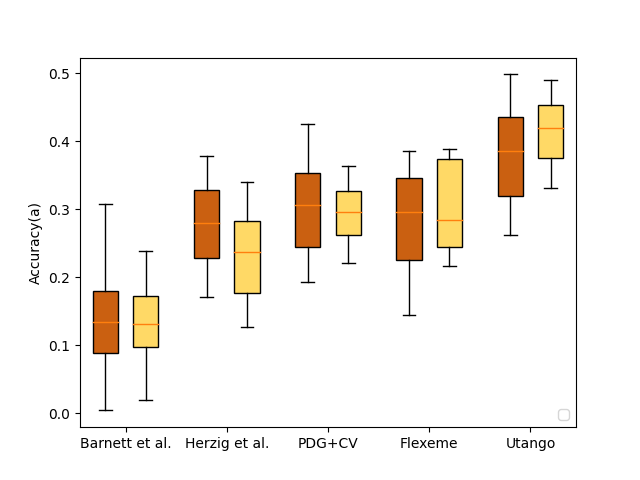
\includegraphics[width=1.7in]{figures/RQ_1_1.png}
                \vspace{-16pt}
		\caption{$Accuracy^c$}
		\label{RQ1-result-3-1}
	\end{subfigure}
	\begin{subfigure}{0.235\textwidth}
		\centering
		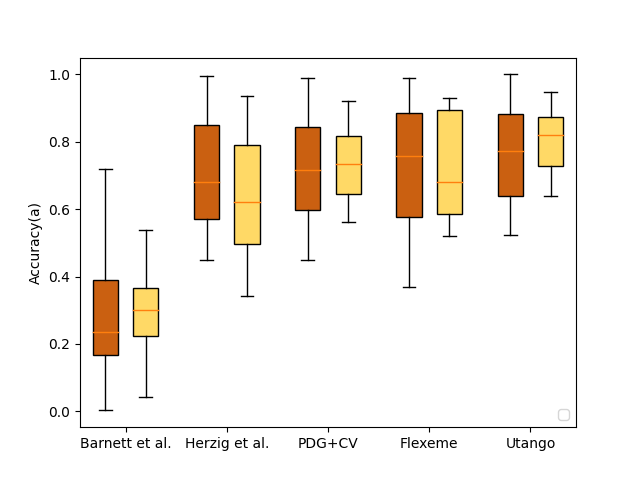
\includegraphics[width=1.7in]{figures/RQ_1_2.png}
                \vspace{-16pt}
		\caption{$Accuracy^a$}
		\label{RQ1-result-3-2}
	\end{subfigure}
        \vspace{-12pt}
	\caption{Boxplots for the Results in Table~\ref{RQ1-result-1} and Table~\ref{RQ1-result-2}. Orange Boxes: 2 concerns data, Yellow Boxes: 3 concerns data}
	\label{RQ1-result-3}
\end{figure}

Figure~\ref{RQ1-result-3} shows the boxplots for both $Accuracy^c$ and
$Accuracy^a$ results in Tables~\ref{RQ1-result-1}
and~\ref{RQ1-result-2}. The orange boxes are for the commits with two
concerns, while the yellow ones are for those with three concerns. As
seen, the median accuracy of {\tool} is higher than those of all
baselines on both types of two and three concerns. Moreover, the gap
between {\tool} and the baselines in $Accuracy^{c}$ is larger than the
gap between them in $Accuracy^{a}$ because all models have correct
classifications by default for the changed statements, which are many
more than the changed ones.

%By considering the average accuracy reported in Table~\ref{RQ1-result-1} and Table~\ref{RQ1-result-2}, \tool has been proved to have the best results on the C\# dataset when compared with all baselines.

%\vspace{3pt}
\noindent {\bf Further Analysis.} For further comparison, we report
that there are {\bf 92} commits that {\tool} correctly classified
100\% of all the changed statements, while there are {\bf 64} commits
that the best baseline, Flexeme, correctly classified all the
changed statements. Both models correctly classified 100\% all the
changed statements of {\bf 13} commits.  Those commits contain from
2--9 changed statements.
       


%do an extra analysis on the number of tangled commits that \tool or the best-performed baseline $Flexeme$ can $100\%$ cluster each changed statement correctly. The results show that there are $92$ commits that \tool can $100\%$ cluster the changed statements correctly while there are $64$ commits that $Flexeme$ can $100\%$ cluster the changed statements correctly. The overlapping between them is about $13$ commits. And the concerns in these commits often have $2-9$ statements inside. The number of commits that \tool can $100\%$ correctly cluster changed statements is limited because there are many concerns in the commits containing many changed statements. It is very hard for \tool to cluster each of them correctly at the same time perfectly. That's also why the concerns in $100\%$ correctly clustered commits often have the limited size from $1$ statements to $9$ statements.

\begin{figure}[t]
	\centering 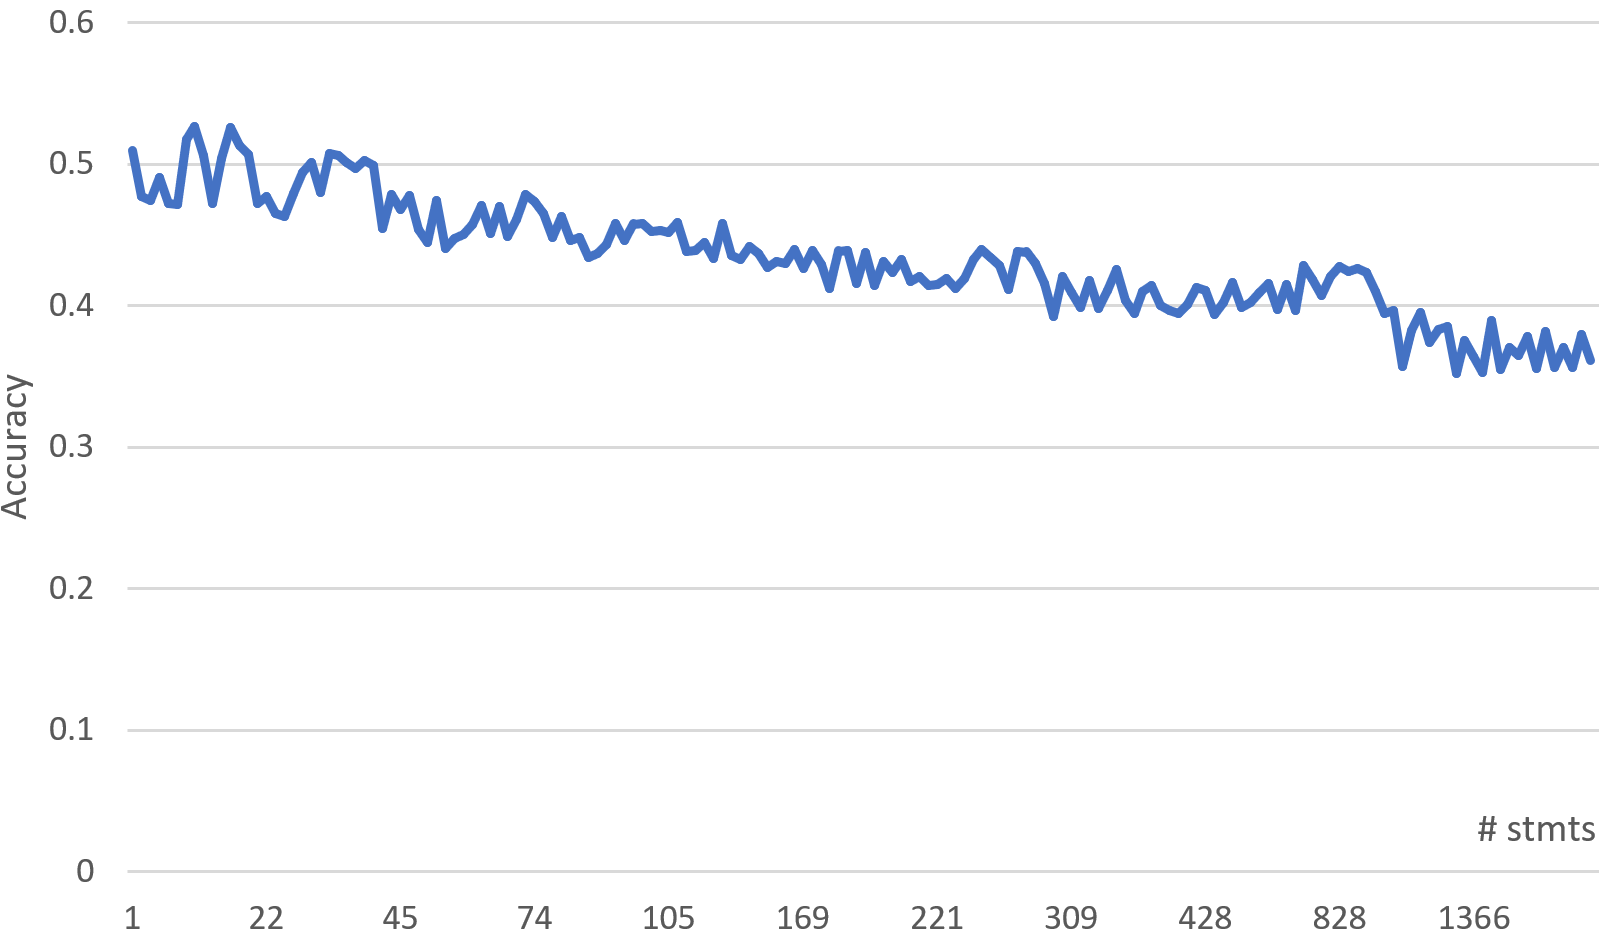
\includegraphics[width=1.8in]{figures/accuracy-concerns.png}
	\vspace{-6pt}
	\caption{Accuracy for Concerns with Diff. Numbers of Stmts}
	\label{acc-concerns}
\end{figure}

To better understand {\tool}'s performance on different sizes of
concerns, we collected all concerns with different numbers of changed
statements and measured the corresponding accuracies for them.  As
seen in Figure~\ref{acc-concerns}, $Accuracy^{c}$ values for the concerns of
small sizes (having 1--22 changed statements) are higher (ranging
from 47\%--54\%). That is, among all the changed statements, {\tool}
correctly classified about 50\% of them into the correct clusters.
For the larger concerns, $Accuracy^{c}$ decreases as expected because
it is more challenging to get correct classifications for more changed
statements in a concern. However, $Accuracy^{c}$ decreases gradually with the
lowest value of around 36\%. Note that there are some commits with the
addition of large files with $>$1.3k lines.

%To better understand the performance of \tool on different sizes of concerns, we collect all concerns, and their size is from $1$ statements to $189$ statements. Then, by dividing them into four groups with the same amount of concerns following the order of the size, \tool can achieve $0.49$, $0.47$, $0.44$, and $0.40$ $Accuracy^c$ on group 1 (with the smallest size of concerns) to group 4 (with the biggest size of concerns), respectively. The results show that \tool can perform slightly better on the smaller size of concerns, but the gap on the results is not too big and still in the acceptable range.


Training of \tool on $80\%$ of C\# dataset takes 1.75 hours and
predicting on $10\%$ of C\# dataset takes 1.3-2.5 seconds for each
commit.


\subsection{{\bf RQ2. Comparative study on Java Dataset}}

\begin{table}[t]
	\caption{RQ2. Comparative study on Java Dataset}
	\vspace{-0.1in}
	\begin{center}
		\footnotesize
		\tabcolsep 4pt
		\renewcommand{\arraystretch}{1} \begin{tabular}{p{1.4cm}<{\centering}|p{0.7cm}<{\centering}p{0.7cm}<{\centering}p{0.7cm}<{\centering}p{1.5cm}<{\centering}|p{0.7cm}<{\centering}}
			
			\hline
			Approaches          & Base-1 & Base-2 & Base-3 & SmartCommit & \tool\\
			\hline
			$Accuracy^{(1)}$   &                &			 	&				   &		&      \\
			\hline
		\end{tabular}
		\label{RQ2-result}
	\end{center}
\end{table}

\subsection{RQ3. Within-Project Analysis}

\begin{table}[t]
	\caption{RQ3. Results for Within- and Mixed-project Settings}
	\vspace{-0.1in}
	\begin{center}
		\footnotesize
		\tabcolsep 4pt
		\renewcommand{\arraystretch}{1} \begin{tabular}{p{2cm}<{\centering}|p{0.8cm}<{\centering}p{0.8cm}<{\centering}p{0.8cm}<{\centering}|p{0.8cm}<{\centering}p{0.8cm}<{\centering}p{0.8cm}<{\centering}}
			
			\hline
			\multirow{2}{*}{Project}     & \multicolumn{3}{c|}{\tool (Within-Project)} & \multicolumn{3}{c}{\tool (Cross-Project)}\\
			\cline{2-7}
			                               &        2       &      3         & Overall  &      2       &        3     & Overall    \\
			
			\hline
			CommandLine (C\#)   &  0.46  & 0.49  &     0.47          &	0.45   & 0.47 &	0.46	       \\
                        netty (Java)   &  0.34  & 0.38  &     0.35          &	0.32   & 0.35 &	0.33	       \\

			\hline
		\end{tabular}
		\label{RQ3-result}
		
	\end{center}
\end{table}


Table~\ref{RQ3-result} shows the comparison between running {\tool} in
the within and cross-project settings. As seen, with sufficient
within-project data, $Accuracy^{c}$ in the within-project setting is
slightly better than that of the mixed-project setting for both
projects in C\# and Java. The trend is consistent for the commits with
2 or 3 concerns. This is expected because the changes in the same
project tend to be more similar than the changes across projects.
This shows that {\tool} works in both within- and mixed-project
settings.

%As we mentioned in the methodology section, because only on the project $Commandline$, \tool can have meaningful results, in Table~\ref{RQ3-result}, all results are only from the project $Commandline$ for a fair comparison. As seen, for $2$ concerns data, $3$ concerns data, and the overall performance, the within project setting can have $2.2\%, 4.3\%,$ and $2.2\%$ higher $Accuracy^c$ compared with the cross-project setting. It shows that using the data from the same project can help the model learn the feature more accurately. However, because the improvement percentages are all less than $5\%$, it proves that \tool can have consistent and similar performance on both the within and cross-project settings.


\subsubsection{{\bf RQ4. Sensitivity Analysis}}


\begin{table}[t]
	\caption{RQ4. Impacts of Key Features on Accuracy}
	\vspace{-12pt}
	\begin{center}
		\footnotesize
		\tabcolsep 4pt
		\renewcommand{\arraystretch}{1} \begin{tabular}{p{3cm}<{\centering}|p{0.8cm}<{\centering}p{0.8cm}<{\centering}p{0.8cm}<{\centering}}
			
			\hline
			       \multirow{2}{*}{}                  & \multicolumn{3}{c}{$Accuracy^c$}\\
			                         \cline{2-4}
			    \# concerns                     & 2 & 3& Overall\\
			\hline

			\tool w/o Context        &  0.38 & 0.43  &   0.40        \\
			\tool w/o Clone Detection     &  0.42 & 0.44  &   0.43        \\
       			\tool                    &  0.44 & 0.47  &   0.45        \\
			\hline
		\end{tabular}
		\label{RQ4-result-1}
	\end{center}
\end{table}

Table~\ref{RQ4-result-1} shows the accuracy results when the key
components in {\tool} were removed. As seen, while both context and
clone detection positively contribute to {\tool}'s accuracy, the
context plays a more important role as expected. Without the context
vector, the accuracy decreases by 13.7\%, 8.5\%, and 11.1\% for the
commits with two, three, and all concerns, respectively. Without the
clone detection, the accuracy decreases by 4.5\%, 6.4\%, and 4.4\% for
the commits with two, three, and all concerns, respectively.

%Table~\ref{RQ4-result-1} shows the changes to the metrics as we remove one key feature from \tool. Generally, each key feature contributes positively to the better performance of {\tool}, as the decreasing of $Accuracy^c$ when removing each of them from \tool. When {\tool} removes context information, the $Accuracy^c$ decreased by $13.7\%, 8.5\%$, and $11.1\%$ on $2$ concerns data, $3$ concerns data, and overall performance, respectively. When {\tool} removes code clone, the $Accuracy^c$ decreased by $4.5\%, 6.4\%$, and $4.4\%$ on $2$ concerns data, $3$ concerns data, and overall performance, respectively.


\begin{table}[t]
	\caption{RQ4. Impact of the Number $k$ of Hops for Context}
	\vspace{-12pt}
	\begin{center}
		\footnotesize
		\tabcolsep 4pt
		\renewcommand{\arraystretch}{1} \begin{tabular}{p{3cm}<{\centering}|p{0.8cm}<{\centering}p{0.8cm}<{\centering}p{0.8cm}<{\centering}}
			
			\hline
			       \multirow{2}{*}{}                  & \multicolumn{3}{c}{$Accuracy^c$}\\
\cline{2-4}
\#concerns & 2 & 3& Overall\\
			\hline
			\tool ($k=1$)          & 0.42 & 0.45 &  0.43          \\
			\tool ($k=2$)          & 0.44 & 0.47 &  0.45          \\
			\tool ($k=3$)          & 0.43 & 0.45 &  0.44          \\
			\tool ($k=4$)          & 0.40 & 0.44 &  0.42          \\
			\tool ($k=5$)          & 0.41 & 0.44 &  0.42          \\
			\tool (Full Graph)     & 0.39 & 0.43 &  0.41          \\
			\hline
		\end{tabular}
		\label{RQ4-result-2}
	\end{center}
\end{table}

Table~\ref{RQ4-result-2} shows the accuracy when we vary the size $K$
of a context (i.e., the number of hops from the changed node). As
seen, when the number of surrounding nodes of the changed node
increases from $K$=1--2, the accuracy increases and reaches its peak
at $K$=2. As $K$=1, the immediate surrounding nodes cannot capture
well the relevant nodes for {\tool} to distinguish the concerns of the
changed statements. With two hops from the changed node, the context
seems to sufficiently contain the crucial nodes w.r.t. determining
the concerns. However, as the size continues to increase, the accuracy
decreases. When the entire graph is used as the context, the accuracy
is the lowest. If more nodes are considered in the context, more noises 
are added as more irrelevant data is used.  The trend is the same for
the commits with two, three, or all concerns.

%Table~\ref{RQ4-result-2} shows that selecting $k$-neighbors for
%context in \tool, $k=2$ is the best choice for \tool because of the
%highest $Accuracy^c$ on $2$ concerns data, $3$ concerns data and
%overall performance. Even though in this table, we only show the $k$
%value range from $1$ to $5$.

%However, from the trend of $Accuracy^c$ changing, we can see that if
%$k>=2$, when $k$ increases, the $Accuracy^c$ decreases with the reason
%that when $k$ increases, the newly added nodes have less relationship
%with the entire node and may bring more biases. Based on this, even
%compared with the untested $k$ value, $k=2$ is still the best setting
%for \tool.

\begin{table}[t]
%	\caption{Top-1 with Data Splitting on CPatMiner dataset}
\caption{Impact of the Size of Training Data}
	\vspace{-12pt}
	\tabcolsep 2pt
	\small
	\begin{center}
\begin{tabular}{|c|l|l|l|}
  \hline
  % after \\: \hline or \cline{col1-col2} \cline{col3-col4} ...
  Splitting on C\# dataset & 80\%/10\%/10\% & 70\%/15\%/15\% & 60\%/20\%/20\% \\
  \hline
  \% $Accuracy^{c}$ & 45\% & 42\% & 37\% \\
  \hline
\end{tabular}
\label{splitting}
	\end{center}
\vspace{-3pt}
\end{table}

As seen in Table~\ref{splitting}, the training data's size has impact
on accuracy. The more training data, the higher the accuracy. Even
reducing it from 80\% to 60\%, {\tool}'s accuracy is still higher than
Flexeme's.


\subsection{RQ5. Analysis on Code Change Embeddings}

To study the projections of the changed statements in the same and
different concerns, we first randomly chose the commits with two or
more clusters/concerns and in one of the cluster/concern, there are at
least two changed statements. Let us use $C$ to denote that
cluster/concern. We randomly chose two changed statements $S_1$ and
$S_2$ in $C$. We then randomly selected another changed statement
$S_3$ such that $S_3 \notin C$ and $S_3$ belongs to another cluster in
the same commit with $S_1$ and $S_2$. We measured the distance
$d_1(S_1,S_2)$ and $d_2(S_1,S_3)$. We repeated the process for all the
commits satisfying the above conditions until to get 384 triples of
($S_1, S_2, S_3$). Based on the population in our dataset, the size of
384 samples gives the confidence level of 95\% and the confidence
interval of 5\%.
%
We used statistical $p$-value to confirm our hypothesis
$H_1: d_1(S_1,S_2)$ $\leq$ $d_2(S_1,S_3)$. The null-hypothesis is
\textit{\textbf{$H_0: d_1(S_1,S_2) > d_2(S_1,S_3)$}}.

When we set the significance level $\alpha = 0.05$, the $p$-value is
$0.03$ (calculated on these 384 samples). In this case, the $p$-value
is smaller than $\alpha$, meaning the null hypothesis would be
rejected at the $\alpha = 0.05$ level. Therefore, our hypothesis
$H_1$: $d_1(S_1,S_2)$$ \leq$$ d_2(S_1,S_3)$ is confirmed.  That is,
the changed statements in the same concerns are projected nearer to
one another than the changed statements in different concerns. This
result is an indication that our {\em context-aware, graph-based embeddings
for code changes are of high quality and helpful in the code change
clustering into different concerns}.

%\textit{\textbf{$H_1: d_1(S_1,S_2) \leq d_2(S_1,S_3)$}}

%Moreover, we also reported the examples where the same changed
%statements in different concerns are projected farther away in the
%vector space.


%To better understand the quality of the code change embeddings, in this RQ, we selected 384 triples of ($S_1, S_2, S_3$) as the statistical analysis sample based on the confidence level of $95\%$ and the confidence interval $5\%$. Our hypothesis for the quality of code change embedding is that $d_1(S_1,S_2)$ $\leq$ $d_2(S_1,S_3)$. 

% which means that our code change embeddings are in good quality.


%\begin{figure}[t]
%	\centering
%	\lstset{
%		numbers=left,
%		numberstyle= \tiny,
%		keywordstyle= \color{blue!70},
%		commentstyle= \color{red!50!green!50!blue!50},
%		frame=shadowbox,
%		rulesepcolor= \color{red!20!green!20!blue!20} ,
%		xleftmargin=1.5em,xrightmargin=0em, aboveskip=1em,
%		framexleftmargin=1.5em,
%		numbersep= 5pt,
%		language=Java,
%		basicstyle=\scriptsize\ttfamily,
%		numberstyle=\scriptsize\ttfamily,
%		emphstyle=\bfseries,
%		moredelim=**[is][\color{red}]{@}{@},
%		escapeinside= {(*@}{@*)}
%	}
%	\begin{lstlisting}[]
%//-----------------------------------Concern-1-------------------------------
%    private void Dispose(bool disposing)
%    {
%(*@{\color{red}{-     \space \space\space\space\space\space\space\space      if% (this.disposed)}@*)
%(*@{\color{cyan}{+    \space\space\space\space\space\space\space\space\space   %     if (disposed)}@*)
%        {
%            return;
%        }
%        ...
%    }
%
%//-----------------------------------Concern-2-------------------------------
%    private HelpText AddOption(string requiredWord, int maxLength, OptionSpecification option, int widthOfHelpText)
%    {
%        ...
%        if (option.ShortName.Length > 0)
%        {
%(*@{\color{red}{-\space\space\space\space\space\space\space\space\space\space  %      if (this.addDashesToOption)}@*)
%(*@{\color{cyan}{+\space\space\space\space\space\space\space\space\space\space %      if (addDashesToOption)}@*)
%	    	{
%			    optionName.Append('-');
%	    	}
%    	...
%    }
%    
%    internal HelpText AddToHelpText(HelpText helpText, bool before)
%    {
%        return before
%(*@{\color{red}{- \space\space\space\space\space\space\space\space               ? this.AddToHelpText(helpText, line => helpText.AddPreOptionsLine(line)) : this.AddToHelpText(helpText, line => helpText.AddPostOptionsLine(line));}@*)
%(*@{\color{cyan}{+  \space\space\space\space\space\space\space\space 	? AddToHelpText(helpText, helpText.AddPreOptionsLine) : AddToHelpText(helpText, helpText.AddPostOptionsLine);}@*)
%    }

%	\end{lstlisting}
%	\vspace{-15pt}
%	\caption{Example for RQ5}
%	\vspace{-6pt}
%	\label{RQ5-example}
%\end{figure}
			
%The code in Figure \ref{RQ5-example} shows an example that contains two concerns. The statement in $Line-4$ in concern-1 is very similar to the statement in $Line-18$ in concern-2. Following the statistical analysis procedure, we pick the statement in $Line-4$ as $S_3$, the statement in $Line-18$ as $S_2$, and the statement in $Line-29$ as $S_1$. Then we calculate the $d_1(S_1,S_2)$ and $d_2(S_1,S_3)$ by using \tool to generate the representation vectors for each changed statement. The results are $d_1(S_1,S_2) = 0.285$ and $d_2(S_1,S_3)=0.491$. This result proves that the similar changed statements in different concerns are projected farther away in the vector space when \tool generates the embedding vectors for the code change statements. It also shows that \tool learns the context information well to distinguish the differences between the similar code changes in a different context.



%\subsection{RQ6. Time Complexity}

Training of \tool on $80\%$ of C\# dataset takes 1.75 hours and predicting on $10\%$ of C\# dataset takes 1.3-2.5 seconds for each commit. Training of \tool on $80\%$ of Java dataset takes XX hours and predicting on $10\%$ of Java dataset takes XX seconds for each commit.


\subsection{Threats to Validity}
\label{threats:sec}

Our study is only on C\# and Java projects. However, the methodology
is language-independent. 


\input{sections/illustrations}



\section{Related Work}
\label{related:sec}

Tangled commits have been reported by several
researchers~\cite{tao-fse12,kim-emse16,kim-msr13,hill-tse12,nguyen-issre13,flexeme-fse20,smartcommit-fse21}. They
have caused negative impacts including hampering code
comprehension~\cite{tao-fse12}, reducing the separation of
concerns~\cite{flexeme-fse20}, and even reducing the accuracy of bug
prediction models that rely on bug-fixing code commits for training.

Recognizing the need of the tools that untangle, i.e., decompose a
commit into untangle changes, several researchers have proposed
different approaches that can be broadly classified into two
categories: {\em mining software repositories}, and {\em program
  analysis}.

First, earlier approaches leverage {\em mining software repositories
  (MSR)} techniques to untangle commits. Herzig {\em et
  al.}~\cite{kim-msr13,kim-emse16} utilize a confidence voter
technique together with agglomerative clustering on the change
operations to untangle the commits.
%Each confidence voter is responsible for an important aspect
%including call-graphs, change couplings, data dependencies, and
%distance measures.
However, the voters are independent, thus, do not reflect well the
interdependency nature of program elements under change. In contrast,
Kirinuki {\em et al.}~\cite{higo-apsec16, higo-icpc14} rely on the
histories of the co-changes to split the tangled code changes before
they are committed. However, they do not consider the relations among
the changes such as data or control dependencies. Dias {\em et
  al.}~\cite{dias-saner15} also use confidence voters, but on the
fine-grained change events in an IDE. The scores are converted into
the similarity ones via a Random Forest Regressor, which are used in
the agglomerative clustering to partition the tangled changes.  The
second category of untangling approaches leverage the {\em static
  analysis} techniques. Roover {\em et al.}~\cite{roover-scam18} use
program slicing to segment a commit across a Program Dependency Graph
(PDG).  However, they are limited in handling interprocedural and
cross-file dependencies. Barnett {\em et al.}~\cite{barnett-icse15}
utilize def-use chains, and cluster them. If the def-use chain all
fall into a method, it is considered as trivial, otherwise,
non-trivial. Because igoring the trivial clusters, it can miss tangled
concerns. To improve over that, Flexeme~\cite{flexeme-fse20} uses
multi-version PDG augmented with name/lexeme flows in the edges, and
applies agglomerative clustering using graph similarity on that graph
to untangle its commits. SmartCommit~\cite{smartcommit-fse21} uses a
graph-partitioning algorithm on a graph representation to capture
different categories of relations among code changes (hard links, soft
links, refactoring links, and cosmetic links).

%check issre2013 for more related work


\newpage

\balance

%\bibliographystyle{plain}
%\bibliographystyle{ACM-Reference-Format}
\bibliographystyle{ACM-Reference-Format}

\bibliography{References}

\end{document}
